%% ============================================================
%% Springer Nature Journal Article
%% Template: sn-jnl.cls (December 2024)
%% Reference style: sn-mathphys-num (numbered, standard for CS/AI)
%%
%% SETUP: Copy sn-jnl.cls and sn-*.bst from the Springer template
%% package into this directory before compiling.
%% Template source:
%%   sn-article-template/sn-article.tex  (December 2024 version)
%%
%% SUBMISSION NOTE: Springer requires a single flat .tex file.
%% Before final submission, inline all \input{} content and remove
%% this instruction block.
%% ============================================================

\documentclass[pdflatex,sn-mathphys-num]{sn-jnl}

%% - Packages -
\usepackage{graphicx}
\usepackage{multirow}
\usepackage{amsmath,amssymb,amsfonts}
\usepackage{booktabs}
\usepackage{algorithm}
\usepackage{algorithmicx}
\usepackage{algpseudocode}
\usepackage{xcolor}
\usepackage{hyperref}

\graphicspath{{./}}
\raggedbottom

%% - Theorem environments (retain for methodology definitions)
\theoremstyle{thmstyleone}
\newtheorem{theorem}{Theorem}
\newtheorem{proposition}[theorem]{Proposition}

\theoremstyle{thmstyletwo}
\newtheorem{example}{Example}
\newtheorem{remark}{Remark}

\theoremstyle{thmstylethree}
\newtheorem{definition}{Definition}

%% =============================================================
\begin{document}
%% =============================================================

%% - Title -
%% Running title (appears in header): keep under 60 characters
\title[SHAP Stability Index for Credit Risk Drift]{%
  SHAP Stability Index as a Leading Indicator of Concept Drift
  in Credit Risk Gradient Boosting Models%
}

%% - Author -
\author*{\fnm{Mohammed} \sur{Azeezulla}}
\email{mmoha134@depaul.edu}

\author{\fnm{Sakshi Balkrishna} \sur{Panpatil}}
\email{spanpati@depaul.edu}

\affil{%
  \orgdiv{College of Computing and Digital Media},
  \orgname{DePaul University},
  \orgaddress{%
    \city{Chicago},
    \state{Illinois},
    \postcode{60604},
    \country{USA}%
  }%
}

%% - Abstract -
%% Rules: unstructured single paragraph, ~200 words,
%%        no citations, no displayed equations, no subheadings.
\abstract{%
Credit risk and fraud models are usually calibrated on historical data, but
production portfolios evolve as borrowers, fraud strategies, and product rules
change. This temporal mismatch can weaken a deployed model before labelled
outcomes are available for validation. Existing monitoring practice mainly
tracks score distributions, input distributions, or realised error rates; it
does not directly ask whether the model's explanation profile has changed. This
paper defines the SHAP Stability Index (SSI), which measures the consistency of
global SHAP feature-importance rankings between adjacent evaluation windows. We
evaluate XGBoost, LightGBM, and CatBoost in a streaming temporal protocol with
ADWIN-triggered adaptive retraining on IEEE-CIS Fraud Detection (590,540
transactions, six months), ULB Credit Card Fraud (284,807 transactions, two
days), and Give Me Some Credit (150,000 records, used as a distributional
stability control). On IEEE-CIS, across 16-17 ADWIN-detected drift events, SSI
falls 7.8 evaluation windows on average (${\text{about }}55$ calendar days) before
AUC degradation is observable (Wilcoxon signed-rank: $p{<}0.001$, $r{=}0.88$
for all three architectures). SSI also separates the observed regimes:
$0.66$-$0.72$ under persistent drift, $0.95$-$0.99$ under localised drift, and
${\mathrel{>=}}0.987$ on the stability control, where it raises no spurious alerts.
SSI is therefore a label-free explanation-stability monitor that complements
performance and distributional checks in credit model governance.%
}

%% - Keywords -
\keywords{concept drift, credit risk, SHAP, model monitoring,
          gradient boosting, feature importance stability}

\maketitle

%% =============================================================
%% =============================================================
%% SECTION 1 - INTRODUCTION
%% No subheadings permitted in Introduction (Springer rule).
%% =============================================================
\section{Introduction}\label{sec:intro}

Machine learning classifiers now support decisions in domains ranging from
medical image diagnosis~\cite{geetha2023skin} to financial services. In credit
risk and fraud detection, the stakes are especially direct: underwriting models
shape access to credit, pricing, expected loss, and fraud intervention. The
Federal Reserve's Model Risk Management guidance (SR~11-7)~\cite{sr117_2011}
therefore requires financial institutions to validate and monitor quantitative
models used for default probability, creditworthiness, and fraud likelihood.
For structured credit data, gradient boosting methods such as
XGBoost~\cite{chen2016xgboost} and LightGBM~\cite{ke2017lightgbm} are widely
used because they perform strongly against logistic regression and neural
network baselines~\cite{lessmann2015credit,shi2022credit}.

Deployment changes the problem. A model is fitted to an earlier sample, while
future borrowers, merchants, fraud tactics, and product policies continue to
move. These changes alter $P(\mathbf{x}, y)$ over time, the setting formalised
as concept drift~\cite{gama2014drift}. The operational risk is not a software
failure but a monitoring failure: predictions can remain available while their
statistical reliability declines. Surveys of financial ML deployments identify
temporal model decay as a major unresolved production
risk~\cite{hinder2024drift,shi2022credit}.

Credit portfolios also suffer from delayed labels. Defaults, charge-offs, and
confirmed fraud outcomes can arrive 30-90 days after the original decision,
so the loss function cannot be measured at the time the decision is made.
Sculley et al.~\cite{sculley2015debt} discuss this delay as a source of
technical debt in deployed ML systems, and Grzenda et
al.~\cite{grzenda2020delayed} show that detection lag for error-based methods
increases with the label-delay window. As a result, detectors such as
ADWIN~\cite{bifet2007adwin}, DDM~\cite{gama2004ddm}, and
EDDM~\cite{baena2006eddm} cannot fire until outcome feedback exists. Label-free
alternatives address only part of the problem. Margin Density Drift Detection
tracks decision-boundary density~\cite{sethi2015margin}, while the Population
Stability Index (PSI)~\cite{siddiqi2006scorecard} tracks marginal score or
feature distributions. Neither directly measures whether the fitted model has
changed its feature reliance while producing apparently stable scores.

A second driver of urgency comes from the regulatory evolution of
interpretability requirements. The European Union Artificial Intelligence
Act~\cite{eu_ai_act2024} classifies credit scoring as a high-risk AI
application subject to mandatory transparency, traceability, and human
oversight requirements throughout the entire operational lifetime of the
model, not just at initial validation. B\"{u}cker et
al.~\cite{bucker2022transparency} showed empirically that the explanatory
quality of deployed credit scoring models depends critically on whether
\emph{explanation consistency} is monitored over time rather than assessed
only at deployment. This creates a dual obligation for credit institutions:
they must detect distributional change early enough to protect predictive
performance, and they must be able to demonstrate that the model's
feature-level decision rationale has not shifted in ways that would compromise
regulatory traceability. Neither obligation is satisfied by existing monitoring
practice.

Explanations provide a second monitoring surface. SHAP (SHapley Additive
exPlanations)~\cite{lundberg2017shap} assigns feature-level contributions to
individual predictions, and TreeSHAP~\cite{lundberg2020trees} computes those
attributions efficiently for tree ensembles. Aggregating absolute SHAP values
over an evaluation window gives a ranked summary of the features driving a
model's decisions for that cohort. Stable rankings imply stable feature
reliance; sharp rank movement implies that the model is using a different
explanatory structure on recent data. Lin and Wang~\cite{lin2025shap} study
SHAP ranking stability in a static credit default model under resampling, but
they do not test whether ranking movement accumulates in a temporal stream or
whether it precedes later performance degradation.

We answer these questions by defining the \textbf{SHAP Stability Index
(SSI)}, computed as the Spearman rank correlation between global SHAP feature
importance vectors in adjacent evaluation windows. When SSI falls, the model is
not merely changing its score distribution; it is changing which variables carry
the decision. That signal is available at scoring time because it uses the
current feature vectors and the fitted model, rather than delayed outcome
labels. SSI therefore fills a monitoring gap left by PSI, error-based drift
detectors, and one-off explanation reviews: it tracks whether the deployed
model's feature reliance remains stable as new data arrive. We test this signal
with XGBoost, LightGBM, and CatBoost on three public credit datasets, using
ADWIN-triggered adaptive retraining and Optuna-based hyperparameter
optimisation~\cite{akiba2019optuna}.

The study contributes the following:

\begin{enumerate}
  \item A temporal evaluation design for credit drift experiments that combines
        three gradient boosting architectures (XGBoost, LightGBM, CatBoost),
        ADWIN drift detection, and Optuna-tuned adaptive retraining across
        three structurally distinct public datasets: IEEE-CIS Fraud Detection
        (590,540 transactions, six months), ULB Credit Card Fraud (284,807
        transactions, two days), and Give Me Some Credit (150,000 records,
        used as a distributional stability control).

  \item The SHAP Stability Index (SSI), a label-free statistic for comparing
        global SHAP importance rankings across successive evaluation windows
        without waiting for ground-truth outcomes.

  \item Evidence that SSI acts as a \emph{leading indicator} on the IEEE-CIS
        stream: across 16-17 ADWIN-detected drift events, SSI declined an
        average of 7.8 evaluation windows (${\text{about }}55$ calendar days) before
        AUC deterioration became detectable, with the same pattern across all
        three model architectures (Wilcoxon $p{<}0.001$, $r{=}0.88$).

  \item Cross-dataset validation showing that the same SSI scale separates
        three regimes: $0.66$-$0.72$ under persistent drift (IEEE-CIS),
        $0.95$-$0.99$ under localised drift (ULB CC Fraud), and
        ${\mathrel{>=}}0.987$ on a distributional stability control (GMSC), without
        threshold recalibration by model family.
\end{enumerate}

The remainder of this paper is organised as follows.
Section~\ref{sec:related} reviews related work on gradient boosting for
credit risk, concept drift detection, and SHAP in financial governance.
Section~\ref{sec:method} formalises the problem and presents the SSI
methodology. Section~\ref{sec:experiments} describes the experimental setup.
Section~\ref{sec:results} presents and discusses the results.
Section~\ref{sec:conclusion} concludes with limitations and future directions.

%% SECTION 2 - RELATED WORK
%% =============================================================
\section{Related Work}\label{sec:related}

\subsection{Gradient Boosting for Credit Risk and Fraud Detection}
\label{sec:related:gb}

Gradient boosting is the main tree-ensemble family used for tabular credit
risk modelling. Chen and Guestrin~\cite{chen2016xgboost} introduced XGBoost,
which combines regularised boosting with column subsampling, shrinkage, and
cache-efficient split enumeration. Ke et al.~\cite{ke2017lightgbm} introduced
LightGBM, replacing depth-wise tree growth with leaf-wise growth and using
gradient-based one-side sampling to reduce the cost of fitting large datasets.
Prokhorenkova et al.~\cite{prokhorenkova2018catboost} introduced CatBoost,
which handles categorical variables through ordered target statistics and
symmetric oblivious trees, reducing target leakage from conventional encoding.
These systems cover the practical design space most relevant to credit risk:
training speed, memory use, and categorical feature handling.

Credit-scoring benchmarks give a consistent reason to focus on these models.
Lessmann et al.~\cite{lessmann2015credit} compared 41 classifiers on eight
public credit datasets and reported that gradient boosting outperformed
logistic regression, neural networks, and support vector machines on both
accuracy and expected-profit measures. Dumitrescu et
al.~\cite{dumitrescu2022credit} showed that non-linear effects learned by
gradient boosting can be incorporated into logistic regression scorecards,
improving accuracy without abandoning interpretable scorecard structure. In a
review of 76 machine-learning credit-risk studies, Shi et
al.~\cite{shi2022credit} likewise identified gradient boosting as a leading
method, while noting that temporal decay and distribution shift remain open
deployment problems.

Credit card fraud detection presents a closely related modelling challenge.
Bhattacharyya et al.~\cite{bhattacharyya2011fraud} demonstrated the superiority
of ensemble methods for fraud classification under severe class imbalance, a
challenge typically addressed through synthetic oversampling~\cite{chawla2002smote}
or cost-sensitive weighting. Bahnsen et al.~\cite{bahnsen2016feature} showed
that temporal and velocity features computed over transaction history are a
primary performance driver beyond point-in-time attributes. Lebichot et
al.~\cite{lebichot2021incremental} demonstrated that incremental learning
strategies can match batch retraining performance in production fraud detection
pipelines operating under concept drift, providing empirical evidence that
adaptive modelling is necessary in non-stationary transaction streams.

Broader tabular benchmarks support the same modelling choice. Shwartz-Ziv and
Armon~\cite{shwartzziv2022tabular} evaluated 48 datasets and found that
tree-based ensembles matched or exceeded neural networks on most tasks,
especially when continuous and categorical variables appear together. Across 45
datasets, Grinsztajn et al.~\cite{grinsztajn2022why} linked this advantage to
irregular feature geometry, a condition under which neural networks still
struggle even after architecture search. Gorishniy et
al.~\cite{gorishniy2021revisiting} reported that transformer architectures for
tabular data do not reliably surpass well-tuned gradient boosting on mixed
feature sets. McElfresh et al.~\cite{mcelfresh2023tabular}, benchmarking 176
datasets and 19 algorithms, found the strongest GBDT advantage on heavy-tailed
or irregular feature distributions, which are common in transaction data.

Beyond accuracy, gradient boosting has attracted scrutiny on fairness and
transparency. Kozodoi et al.~\cite{kozodoi2022fairness} demonstrated that
fairness-aware models can achieve competitive AUC while measurably reducing
discriminatory outcomes, at the cost of a quantifiable profit trade-off.
B{\"u}cker et al.~\cite{bucker2022transparency} concluded that the explanatory
quality of deployed credit scoring models depends critically on whether
explanation consistency is monitored over time rather than assessed only at
initial validation - a finding that directly motivates the SSI framework.

These benchmarks are informative but mostly static. They do not test how the
same models behave after deployment, when the evaluation stream keeps moving
and the relationship between features and outcomes can change. The experiments
in Section~\ref{sec:experiments} are designed around that temporal setting.

\subsection{Concept Drift Detection in Data Streams}
\label{sec:related:drift}

Concept drift refers to changes in the joint distribution $P(\mathbf{x}, y)$
over time that reduce the predictive validity of a trained model. Gama et
al.~\cite{gama2014drift} provided the foundational taxonomy, distinguishing
gradual, abrupt, incremental, and recurring drift together with a unified review
of detection and adaptation strategies. Webb et al.~\cite{webb2016drift} refined
this taxonomy by separating virtual drift, in which only the marginal
$P(\mathbf{x})$ shifts, from real drift, in which the posterior
$P(y \mid \mathbf{x})$ changes. The distinction has practical consequences:
virtual drift may not require retraining, whereas real drift requires model
adaptation to maintain predictive validity.

\paragraph{Statistical drift detectors.}
Performance-based detectors watch an online error stream and declare drift when
recent errors no longer look consistent with earlier errors. ADWIN (Adaptive
WINdowing)~\cite{bifet2007adwin} keeps a variable-length window and cuts it
when two subwindows differ enough to satisfy its statistical test.
DDM~\cite{gama2004ddm} instead compares the current error process with its best
historical point, while EDDM~\cite{baena2006eddm} shifts the focus from error
rate to the spacing between errors to improve sensitivity under gradual drift.
Other detectors monitor different signals: KSWIN~\cite{raab2020kswin} applies a
Kolmogorov-Smirnov comparison to recent univariate observations,
HDDM~\cite{frias2015hddm} uses Hoeffding-test warning and drift levels, and the
Page-Hinkley test~\cite{page1954phtest} accumulates directional deviations in a
scalar sequence.

These methods are useful but not interchangeable. They differ in how quickly
they react, how often they false alarm, and whether labels are required. We use
ADWIN because its adaptive window fits the bursty drift pattern expected in
transaction streams and because River~\cite{montiel2021river} provides a stable
implementation that can be embedded directly into the evaluation loop.

\paragraph{Adaptive learning and monitoring frameworks.}
Street and Kim~\cite{street2001streaming} proposed ensemble-based streaming
classifiers that retire stale component models and train new ones at block
boundaries, implicitly handling gradual drift. Losing et
al.~\cite{losing2018incremental} reviewed incremental online learning methods
and found that detector-triggered full retraining outperforms passive forgetting
under abrupt drift - precisely the regime ADWIN is designed to identify.
Klaise et al.~\cite{klaise2020monitoring} formalised the case for integrating
drift detection, outlier detection, and explanation monitoring as complementary
components of a single production observability pipeline, noting that no single
signal is sufficient in isolation.

\paragraph{Surveys and the detection gap.}
Bayram et al.~\cite{bayram2022drift} reviewed performance-aware drift detectors
and confirmed that all current methods measure model degradation that has already
manifested in prediction errors rather than anticipating it from upstream
signals. The 2024 two-part survey by Hinder et al.\ addresses both the detection
question~\cite{hinder2024drift} and the drift localisation and explanation
question~\cite{hinder2024partb}, collectively identifying the temporal gap
between drift onset and detector response as the central open problem in the
field. Lu et al.~\cite{lu2018drift} reviewed learning-under-drift approaches
across domains and noted that interpretability of drift causes remains largely
absent from the literature.

\paragraph{Production monitoring in financial machine learning.}
In credit model monitoring, the Population Stability Index (PSI) is commonly
used to compare a reference population with a later monitoring
population~\cite{siddiqi2006scorecard}. It bins a score or feature into $n$
intervals and computes:
\begin{equation}
  \mathrm{PSI} = \sum_{i=1}^{n}
    \bigl(A_i - E_i\bigr)\ln\!\Bigl(\tfrac{A_i}{E_i}\Bigr),
  \label{eq:psi}
\end{equation}
where $A_i$ and $E_i$ denote monitoring and reference proportions in bin $i$.
Values above 0.25 are typically treated as requiring review under
SR~11-7~\cite{sr117_2011}. The Characteristic Stability Index (CSI) applies the
same calculation feature by feature. PSI and CSI are therefore well suited to
distribution checks, but their unit of analysis is still a marginal
distribution. They do not say whether the fitted model is relying on the same
features for its decisions. SSI is introduced for that missing internal-logic
signal.

\paragraph{The label delay problem.}
In production credit systems, labels often arrive after the monitoring decision
is needed. Sculley et al.~\cite{sculley2015debt} describe label delay and model
decay as technical debt in deployed ML systems. Sethi and
Kantardzic~\cite{sethi2015margin} avoid immediate label dependence by monitoring
the density of observations near the classifier margin, and Grzenda et
al.~\cite{grzenda2020delayed} show that error-based drift detection slows as the
delay window grows. SSI follows the same operational constraint: it uses the
current feature vectors and fitted model at inference time, not resolved
outcomes.

\subsection{Explainable AI in Credit Risk Governance}
\label{sec:related:xai}

Interpretability in consumer credit is now part of model governance, not only a
post-hoc reporting preference. SR~11-7~\cite{sr117_2011} requires ongoing model
validation and monitoring, while the Basel Committee's operational risk
principles~\cite{basel2011} impose related transparency expectations for models
used in capital contexts. The European Union Artificial Intelligence
Act~\cite{eu_ai_act2024} treats credit scoring as a high-risk AI use case,
bringing traceability and human oversight into the operating life of the model.
If a model's SHAP importance rankings move sharply over time, the explanation
record available to auditors has changed even when aggregate AUC remains
acceptable.

Two post-hoc explanation methods are especially common in financial ML.
LIME~\cite{ribeiro2016lime} fits a local surrogate around an individual prediction.
SHAP~\cite{lundberg2017shap} assigns Shapley-value attributions to features,
with efficiency, symmetry, dummy, and linearity properties. Subsequent work shows
why these explanations require care: Sundararajan and
Najmi~\cite{sundararajan2020shapley} analyse how the Shapley-value
operationalisation and background distribution affect attributions, while Covert
et al.~\cite{covert2021removing} place SHAP, LIME, and permutation importance in
a shared removal-based framework. TreeSHAP~\cite{lundberg2020trees} is the
relevant variant here because it computes exact attributions for tree ensembles
efficiently. Arrieta et al.~\cite{arrieta2020xai} identify temporal consistency
as an open XAI issue, but most stability studies still evaluate one trained
model under perturbations rather than a model deployed through a changing stream.

The stability and fragility of post-hoc explanations have been examined from
several angles with direct governance implications. Alvarez-Melis and
Jaakkola~\cite{alvarez2018robustness} defined a self-consistency criterion
requiring that similar inputs produce similar explanations and showed that neither
LIME nor SHAP satisfies it uniformly, establishing precedent for treating
explanation stability as a measurable governance property. Slack et
al.~\cite{slack2020fooling} demonstrated that both methods can be adversarially
manipulated to conceal discriminatory behaviour behind innocuous-looking
explanations, underscoring that static explanation audits are insufficient for
deployed systems under distribution shift. Fryer et al.~\cite{fryer2021shapley}
showed that Shapley values for feature selection can produce misleading importance
rankings under correlated features - a common condition in credit data -
indicating that attribution instability is a concern even before distributional
shift is introduced. Molnar et al.~\cite{molnar2022pitfalls} catalogued general
pitfalls of model-agnostic interpretation methods, including failure to account
for feature dependence and production of spurious attributions in high-dimensional
settings, concluding that one-time explanation audits provide insufficient
governance coverage for production systems.

In the credit domain specifically, Bussmann et al.~\cite{bussmann2021credit}
integrated SHAP attribution monitoring into an end-to-end credit risk management
framework, treating SHAP values as first-class governance artefacts alongside
AUC and Gini coefficient and demonstrating the practical utility of feature-level
explanation tracking in production. Guidotti et al.~\cite{guidotti2018survey}
identified explanation stability as a key desideratum alongside fidelity,
observing that explanations which change arbitrarily between consecutive decision
windows provide no actionable governance signal. Molnar~\cite{molnar2022iml}
discusses global feature importance consistency as a practical property analysts
should assess but provides no quantitative framework for monitoring it over time.

The most directly related prior work is Lin and Wang~\cite{lin2025shap}, who
examined SHAP ranking stability in a static credit card default model across
resampling strategies and class imbalance conditions, finding significant rank
variation across experimental configurations. Their study is restricted to a
single cross-sectional model under controlled perturbations and does not examine
whether SHAP rankings shift systematically across temporal evaluation windows as
concept drift accumulates, nor whether such shifts carry predictive information
about upcoming performance degradation before it surfaces in outcome metrics.
These are precisely the questions addressed by the SHAP Stability Index
introduced in Section~\ref{sec:method}.

%% SECTION 3 - METHODOLOGY
%% =============================================================
\section{Methodology}\label{sec:method}

\subsection{Problem Formulation}\label{sec:method:problem}

Let $\mathcal{D} = \{(\mathbf{x}_t, y_t)\}_{t=1}^{T}$ denote a temporal stream
of credit transactions, where $\mathbf{x}_t \mathbin{\mathrm{in}} \mathbb{R}^d$ is the feature
vector at time $t$ and $y_t \mathbin{\mathrm{in}} \{0, 1\}$ is the binary outcome label. We
partition $\mathcal{D}$ into $K$ non-overlapping evaluation windows
$W_1, W_2, \ldots, W_K$ of fixed size $w$ with stride $s$, preserving temporal
order so that no future observations enter any window's training set.

At each window $k$, a gradient boosting model $\mathcal{M}_k$ is trained on all
data preceding $W_k$ and evaluated on $W_k$. Two regimes are compared throughout
this study:
\begin{itemize}
  \item \textbf{Static}: $\mathcal{M}_k = \mathcal{M}_1$ for all $k$; the model
        is trained once at initialisation and never updated after deployment.
  \item \textbf{Adaptive}: $\mathcal{M}_k$ is retrained whenever an online drift
        detector signals a statistically significant change in the model's error
        rate.
\end{itemize}

A concept drift event occurs at window $k$ when the joint distribution
$P_k(\mathbf{x}, y)$ differs significantly from $P_{k-1}(\mathbf{x}, y)$ as
determined by ADWIN~\cite{bifet2007adwin}. Real drift, in which the conditional
$P_k(y \mid \mathbf{x})$ shifts, degrades the static model's predictions
systematically, whereas the adaptive model recovers by retraining on the most
recent data.

\subsection{The SHAP Stability Index}\label{sec:method:ssi}

At each evaluation window $k$, TreeSHAP~\cite{lundberg2020trees} is applied to
a stratified subsample of up to 2,000 instances drawn from $W_k$. TreeSHAP
computes exact Shapley values for tree ensembles in polynomial time without the
exponential enumeration required by the general Shapley formula, making it
tractable for high-dimensional credit datasets evaluated repeatedly across
many windows.

The global feature importance vector $\mathbf{s}_k \mathbin{\mathrm{in}} \mathbb{R}^d$
is defined component-wise as the mean absolute SHAP value across the sampled
instances:
\begin{equation}
  s_k^{(j)} = \frac{1}{|S_k|}
    \sum_{i \mathbin{\mathrm{in}} S_k} \bigl|s_j(\mathbf{x}_i)\bigr|,
  \qquad j = 1, \ldots, d,
  \label{eq:global_shap}
\end{equation}
where $S_k \mathbin{\mathrm{inside}} W_k$ is the evaluation sample and $s_j(\mathbf{x}_i)$
is the SHAP attribution for feature $j$ on instance $\mathbf{x}_i$. Let
$\mathbf{R}_k \mathbin{\mathrm{in}} \mathbb{Z}^{d'}$ denote the rank vector obtained by ordering
the top $d' = 20$ components of $\mathbf{s}_k$ in descending order.
Restricting to the top-$d'$ features reduces noise from low-importance features
whose ranks fluctuate arbitrarily near the tail of the distribution.

\begin{definition}[SHAP Stability Index]
\label{def:ssi}
The \textbf{SHAP Stability Index} at window $k$ with lookback $L$ is:
\begin{equation}
  \mathrm{SSI}(k)
    = \frac{1}{L} \sum_{h=1}^{L}
        r_s\!\left(\mathbf{R}_{k-h+1},\, \mathbf{R}_{k-h}\right),
  \label{eq:ssi}
\end{equation}
where $r_s$ denotes the Spearman rank correlation coefficient.
\end{definition}

Spearman correlation is used in preference to Pearson correlation because SHAP
magnitudes vary in scale across windows independently of rank structure; the
ordinal measure captures genuine reordering while remaining invariant to
monotone rescaling of attribution values. $\mathrm{SSI}(k) = 1$ indicates an
identical feature importance ordering to the preceding window; values near zero
indicate a near-random rearrangement. SSI requires only model outputs and
unlabelled feature vectors and can therefore be computed at inference time
before ground-truth labels become available.

\paragraph{SSI as a leading indicator.}
For each ADWIN-detected drift event, we measure the lead time $L_{\mathrm{lead}}$ of SSI
relative to AUC degradation by defining three quantities:
\begin{itemize}
  \item $k_{\mathrm{SSI}}$: the first window at which
        $\mathrm{SSI}(k) < T_{\mathrm{SSI}}$, where the instability
        threshold $T_{\mathrm{SSI}} = 0.80$.
  \item $k_{\mathrm{AUC}}$: the first window after drift onset at which the
        AUC falls more than $D_{\mathrm{AUC}} = 0.02$ below the pre-drift baseline.
  \item Lead time: $L_{\mathrm{lead}} = k_{\mathrm{AUC}} - k_{\mathrm{SSI}}$ (in
        evaluation windows). A positive value indicates that SSI signalled
        instability before AUC degradation was detectable.
\end{itemize}

\paragraph{Parameter selection rationale.}
The SSI hyperparameters $d'$, $L$, and $T_{\mathrm{SSI}}$ are motivated
as follows.

\textbf{Top-$d'$ truncation ($d' = 20$).} In gradient boosting models for
tabular credit data, feature importance follows a heavy-tailed distribution:
a small number of features accounts for the majority of total mean absolute
SHAP attribution, while the tail consists of near-zero contributions whose
rank order fluctuates arbitrarily from window to window. Restricting SSI to
the top $d' = 20$ features by mean absolute SHAP value focuses the rank
correlation on the semantically meaningful portion of the importance ordering
and removes the noise introduced by features operating near zero attribution.
The value $d' = 20$ is chosen to exceed the approximate ``elbow'' in the
SHAP importance distribution observed during exploratory analysis of the
IEEE-CIS dataset, beyond which additional features contribute negligible
marginal attribution.

\textbf{Lookback window ($L = 5$).} The lookback $L$ determines the temporal
span of the rolling average in Equation~\eqref{eq:ssi}. With the 7-day
evaluation stride on IEEE-CIS, $L = 5$ yields a 35-day effective monitoring
window, matching the sub-monthly review horizon at which model risk governance
processes are typically active in credit institutions. Values $L < 3$ produce
a volatile one-shot measure sensitive to single-window noise; values $L > 7$
introduce excessive lag that would delay detection of abrupt drift episodes.
$L = 5$ balances responsiveness with noise suppression.

\textbf{Instability threshold ($T_{\mathrm{SSI}} = 0.80$).} The threshold
determines which SSI values are classified as indicating feature-ranking
instability. A sensitivity analysis reported in
Section~\ref{sec:res:sensitivity} demonstrates that SSI's first crossing
below threshold is invariant to $T$ over the range $[0.66, 0.90]$ for both
model families on the IEEE-CIS dataset: all values in this range detect the
onset of instability at the same evaluation window. Values below 0.65 reduce
coverage to fewer than 30\% of the drift-affected windows. The chosen
$T_{\mathrm{SSI}} = 0.80$ lies in the middle of the stable detection range
and is consistent with Spearman correlation thresholds used in analogous rank
stability audits in the psychometric literature.

\subsection{ADWIN-Triggered Adaptive Retraining}\label{sec:method:adwin}

ADWIN maintains a self-adjusting window $W$ over a scalar performance signal,
specifically the per-window classification error rate $(1 - \text{accuracy})$.
At each step, ADWIN tests whether the mean of any contiguous sub-window
$W_0 \mathbin{\mathrm{inside}} W$ differs significantly from the mean of the complement
$W_1 = W \setminus W_0$:
\begin{equation}
  \bigl|m_{W_0} - m_{W_1}\bigr| \mathrel{>=} e_{\mathrm{cut}},
  \label{eq:adwin}
\end{equation}
where $e_{\mathrm{cut}}$ is derived from the Hoeffding bound at
confidence level $1 - d_{\mathrm{ADWIN}}$~\cite{bifet2007adwin}. The window is trimmed
from its oldest end until no such partition satisfies
Equation~\eqref{eq:adwin}. When a cut is found, a drift event is declared and
the adaptive model is retrained immediately. The ADWIN implementation is
provided by the River streaming machine learning library~\cite{montiel2021river},
which is consistent with the original algorithm specification~\cite{bifet2007adwin}.

Algorithm~\ref{alg:streaming} describes the complete streaming evaluation loop
applied to every dataset and model combination in this study.

\begin{algorithm}[t]
\caption{Temporal Streaming Evaluation with ADWIN and SSI Monitoring}
\label{alg:streaming}
\begin{algorithmic}[1]
  \Require Windows $W_1,\ldots,W_K$; model $\mathcal{M}$;
           $\mathrm{ADWIN}(d_{\mathrm{ADWIN}})$; lookback $L$; buffer size $B$
  \State Train $\mathcal{M}$ on windows $W_1,\ldots,W_{\mathrm{init}}$
  \State Initialise training buffer
         $\mathcal{B} \leftarrow \{W_1,\ldots,W_{\mathrm{init}}\}$
  \For{$k = \mathrm{init}+1$ \textbf{to} $K$}
    \State Compute $\mathrm{AUC}_k$, $\mathrm{error}_k$ on $W_k$ using
           $\mathcal{M}$
    \State Feed $\mathrm{error}_k$ to $\mathrm{ADWIN}(d_{\mathrm{ADWIN}})$
    \State Compute $\mathbf{s}_k$ via TreeSHAP on stratified sample
           of $W_k$
    \State Compute $\mathrm{SSI}(k)$ via Equation~\eqref{eq:ssi}
    \If{$\mathrm{ADWIN}$ signals drift}
      \State Retrain $\mathcal{M}$ on the $B$ most recent windows in
             $\mathcal{B}$
      \State Log: $k$, $\mathrm{AUC}_k$, $\mathrm{SSI}(k)$, lead time
             $L_{\mathrm{lead}}$
    \EndIf
    \State Add $W_k$ to $\mathcal{B}$; drop oldest window if
           $|\mathcal{B}| > B$
  \EndFor
  \State \Return $\{\mathrm{AUC}_k\}_k$, $\{\mathrm{SSI}(k)\}_k$,
         drift event log
\end{algorithmic}
\end{algorithm}

\subsection{Hyperparameter Optimisation}\label{sec:method:optuna}

XGBoost, LightGBM, and CatBoost are each tuned using
Optuna~\cite{akiba2019optuna} with the Tree-structured Parzen Estimator (TPE)
sampler~\cite{bergstra2011tpe}. TPE
models the distribution of hyperparameters that produced high-performing trials
as one Gaussian mixture density $p_{\mathrm{good}}(z)$, and that of
low-performing trials as another, $p_{\mathrm{bad}}(z)$, then samples
candidates where the ratio $p_{\mathrm{good}}(z)/p_{\mathrm{bad}}(z)$ is
maximised. This concentrates search effort in promising regions without
requiring a global surrogate regression model.

The tuning objective is AUC evaluated on a held-out temporal validation window
$W_{\mathrm{val}}$ placed immediately after the training period, ensuring that
no future data influences hyperparameter selection. Each tuning run executes
150 trials subject to a two-hour wall-clock timeout. The Median pruner
terminates unpromising trials whose intermediate AUC on $W_{\mathrm{val}}$
falls below the median of completed trials at the same optimisation step.
All optimised hyperparameter sets are serialised as JSON files for exact
reproducibility. The full parameter search spaces for each model are listed
in Section~\ref{sec:experiments}.


%% =============================================================
%% SECTION 4 - EXPERIMENTAL SETUP
%% =============================================================
\section{Experimental Setup}\label{sec:experiments}

\subsection{Datasets}\label{sec:exp:data}

Three publicly available datasets spanning distinct credit risk and fraud
detection tasks are used to evaluate the proposed framework.
Table~\ref{tab:datasets} summarises their key characteristics.

\textbf{IEEE-CIS Fraud Detection.} This dataset contains 590,540 card
transactions provided as two source files, transaction attributes and identity
metadata, joined on a shared transaction identifier. The binary label
\texttt{isFraud} is imbalanced at approximately 3.5\% positive. The merged raw
feature space exceeds 400 columns, comprising the transaction amount, 14 count
features (\texttt{C1}-\texttt{C14}), 15 time-delta features (\texttt{D1}-\texttt{D15}),
nine binary match flags (\texttt{M1}-\texttt{M9}), 339 anonymised \texttt{V}-features,
card identifiers, and device identity attributes. A real calendar timestamp
(\texttt{TransactionDT}, in seconds relative to a reference date) enables
genuine temporal ordering across a six-month collection period.


\textbf{Give Me Some Credit (GMSC) - distributional stability control.}
This dataset contains 150,000 borrower records with binary label
\texttt{SeriousDlqin2yrs} (${\text{about }}6.7$\% positive) and 10 credit-bureau
features. It contains no real timestamp. A pseudo-temporal ordering is
constructed by sorting on age (ascending) then revolving utilisation
(descending), which creates a smooth demographic gradient rather than a
genuine temporal sequence. GMSC is included exclusively as a
\emph{distributional stability control} (negative control): it tests
whether SSI produces spurious low-stability alerts when data are ordered by
demographic attributes rather than time. Any observation of high SSI
(${\mathrel{>=}}0.987$) and zero ADWIN events on GMSC is expected by design and
cannot be cited as drift-detection validation; it confirms only that the
metric does not false-positive on smoothly demographically ordered data.

\textbf{ULB Credit Card Fraud - localised-drift control.}
This well-studied benchmark~\cite{dalpozzolo2015ccfraud}
contains 284,807 European card transactions recorded over two calendar days in
September 2013. The binary label \texttt{Class} indicates fraud (492 events,
0.17\%). Features \texttt{V1}-\texttt{V28} are principal components of
anonymised transaction attributes; only \texttt{Time} (elapsed seconds since
the first transaction) and \texttt{Amount} are provided in raw form. Its
two-day span yields a single ADWIN drift event, making it a localised-drift
control rather than a persistent-drift experiment.

\begin{table}[t]
  \caption{Summary of the three evaluation datasets. Positive rate is the
           fraction of fraudulent or delinquent instances. Engineered feature
           counts reflect the final dimensionality after all transforms and
           selection steps described in Section~\ref{sec:exp:features}.
           GMSC has no real timestamp and is used as a distributional
           stability control only.}
  \label{tab:datasets}
  \centering\footnotesize
  \begin{tabular}{@{}lrrrrcl@{}}
    \toprule
    Dataset & Records & Raw & Eng. & Pos.\ (\%) & Span & Temporal Basis \\
    \midrule
    IEEE-CIS Fraud      & 590,540 & $>$400 & 200 & 3.5  & 6 mo. & TransactionDT \\
    GMSC                & 150,000 & 10     &  17 & 6.7  & N/A   & Stability control \\
    ULB CC Fraud        & 284,807 & 30     &  38 & 0.17 & 2 d.  & Time (s)      \\
    \bottomrule
  \end{tabular}
\end{table}

\subsection{Feature Engineering}\label{sec:exp:features}

All feature transforms are fitted exclusively on data preceding each evaluation
window and applied without re-fitting to that window, eliminating any
look-ahead leakage across the temporal boundary.

\textbf{IEEE-CIS.} \texttt{TransactionAmt} yields three derived predictors:
log-transform, decimal-part extraction, and a binary round-amount flag.
Calendar features (day of week, hour of day, weekend indicator) are decoded
from the \texttt{TransactionDT} timestamp. Transaction amounts are aggregated
within seven cardholder-group columns (\texttt{card1}-\texttt{card6},
purchaser email domain) to produce per-group count, mean, standard deviation,
and maximum statistics. Each of the 15 \texttt{D}-columns receives a
log-transform and a binary missing-value indicator. Highly correlated
\texttt{V}-feature pairs (Pearson $r > 0.95$ on training data) are removed to
eliminate multicollinearity. Categorical columns, including product code, card network,
email domain, match flags, and device type, are target-encoded with Laplace
smoothing (prior weight $k = 300$). Identity fields
(\texttt{id\_01}-\texttt{id\_38}) are label-encoded with an explicit
\textit{unknown} token to handle categories unseen in evaluation windows.
Residual missing numerical values are imputed with $-999$. A LightGBM
relevance filter retains the top 200 features by training-set Gini importance,
yielding a final 200-dimensional representation.


\textbf{ULB CC Fraud.} \texttt{Amount} is log-transformed, z-scored using
training-partition statistics, and a round-amount indicator is added.
The \texttt{Time} field produces hour-of-day, day-of-period, and a night-hours
indicator (00:00-06:00). Five pairwise products among the first four principal
components (\texttt{V1}-\texttt{V4}) are appended as interaction features,
yielding 38 dimensions in total.

\textbf{GMSC.} Age values of zero are replaced by the training-partition
median. Delinquency counts are capped at 90. Four derived features are
added: total late payments, debt-to-income ratio, income per dependent,
and credit utilisation risk. Monthly income receives a log-transform and
age is discretised into six bands. A pseudo-time index is appended.
Final dimension: 17 features.

Class imbalance is addressed via SMOTE~\cite{chawla2002smote} applied
\emph{within the training partition only} at each (re)training step for
IEEE-CIS and GMSC; SMOTE is never applied to evaluation windows.
For ULB CC Fraud, the extreme rarity of positive instances ($<$0.2\%) is
handled through cost-sensitive learning via the class-weight mechanism of
each model, which avoids the computational overhead of synthetic oversampling
on a continuous input space already transformed by PCA.

\subsection{Temporal Evaluation Protocol}\label{sec:exp:temporal}

Each dataset is partitioned into non-overlapping evaluation windows following
the strategy formalised in Section~\ref{sec:method:problem}. All windowing
parameters are fixed before model training and held constant across the static
and adaptive variants, ensuring a controlled comparison.
Table~\ref{tab:windows} lists the parameters. Both datasets use
calendar-duration windows aligned to their respective temporal granularity.

\begin{table}[t]
  \caption{Temporal windowing parameters for each dataset. The minimum
           training windows column denotes how many windows must accumulate
           before the first evaluation window is scored.}
  \label{tab:windows}
  \centering
  \begin{tabular}{lllrr}
    \toprule
    Dataset & Window & Stride & Min.\ Train & Eval.\ Windows \\
    \midrule
    IEEE-CIS     & 14 days      & 7 days       & 6  & 18 \\
    GMSC         & 1/20 data    & 1/20 data    & 8  & 12 \\
    ULB CC Fraud & 4 hours      & 2 hours      & 4  & $\text{about }$19 \\
    \bottomrule
  \end{tabular}
\end{table}

The ADWIN confidence parameter is set to $d_{\mathrm{ADWIN}} = 0.002$ and the retraining
buffer to $B = 5$ most recent windows. SSI is computed with lookback $L = 5$
and monitors the top $d' = 20$ features as defined in
Equation~\eqref{eq:ssi}, with instability threshold
$T_{\mathrm{SSI}} = 0.80$.

\subsection{Hyperparameter Search Spaces}\label{sec:exp:hparams}

Tables~\ref{tab:xgb_space}, \ref{tab:lgb_space}, and~\ref{tab:cb_space}
list the Optuna search spaces used for XGBoost, LightGBM, and CatBoost
respectively. All three studies use the TPE sampler~\cite{bergstra2011tpe}
(seed 42) with the Median pruner (20 start-up trials, 5 warm-up steps each).
Each study runs for up to 150 trials subject to a two-hour wall-clock
timeout. The tuning objective is AUC evaluated on the temporal validation
window $W_{\mathrm{val}}$ placed immediately after the initial training
period.

\begin{table}[t]
  \caption{XGBoost hyperparameter search space.}
  \label{tab:xgb_space}
  \centering
  \begin{tabular}{lll}
    \toprule
    Parameter & Range / Values & Sampling \\
    \midrule
    \texttt{n\_estimators}       & \{50, 75, \ldots, 300\}  & Discrete (step 25) \\
    \texttt{max\_depth}          & {[}3, 9{]}               & Discrete uniform \\
    \texttt{learning\_rate}      & {[}0.01, 0.30{]}         & Log-uniform \\
    \texttt{min\_child\_weight}  & {[}1, 20{]}              & Discrete uniform \\
    \texttt{subsample}           & {[}0.5, 1.0{]}           & Uniform \\
    \texttt{colsample\_bytree}   & {[}0.3, 1.0{]}           & Uniform \\
    \texttt{colsample\_bylevel}  & {[}0.3, 1.0{]}           & Uniform \\
    \texttt{reg\_alpha}          & {[}$10^{-8}$, 10{]}      & Log-uniform \\
    \texttt{reg\_lambda}         & {[}$10^{-8}$, 10{]}      & Log-uniform \\
    \texttt{gamma}               & {[}0.0, 5.0{]}           & Uniform \\
    \texttt{scale\_pos\_weight}  & {[}1, 100{]}             & Discrete uniform \\
    \bottomrule
  \end{tabular}
\end{table}

\begin{table}[t]
  \caption{LightGBM hyperparameter search space.}
  \label{tab:lgb_space}
  \centering
  \begin{tabular}{lll}
    \toprule
    Parameter & Range / Values & Sampling \\
    \midrule
    \texttt{n\_estimators}      & \{200, 250, \ldots, 1500\} & Discrete (step 50) \\
    \texttt{num\_leaves}        & {[}20, 200{]}              & Discrete uniform \\
    \texttt{max\_depth}         & {[}3, 12{]}                & Discrete uniform \\
    \texttt{learning\_rate}     & {[}0.01, 0.30{]}           & Log-uniform \\
    \texttt{min\_child\_samples}& {[}5, 100{]}               & Discrete uniform \\
    \texttt{subsample}          & {[}0.5, 1.0{]}             & Uniform \\
    \texttt{subsample\_freq}    & {[}1, 10{]}                & Discrete uniform \\
    \texttt{colsample\_bytree}  & {[}0.3, 1.0{]}             & Uniform \\
    \texttt{reg\_alpha}         & {[}$10^{-8}$, 10{]}        & Log-uniform \\
    \texttt{reg\_lambda}        & {[}$10^{-8}$, 10{]}        & Log-uniform \\
    \texttt{min\_split\_gain}   & {[}0.0, 1.0{]}             & Uniform \\
    \texttt{is\_unbalance}      & \{True, False\}            & Categorical \\
    \bottomrule
  \end{tabular}
\end{table}

\begin{table}[t]
  \caption{CatBoost hyperparameter search space.}
  \label{tab:cb_space}
  \centering
  \begin{tabular}{lll}
    \toprule
    Parameter & Range / Values & Sampling \\
    \midrule
    \texttt{iterations}          & \{200, 250, \ldots, 1500\} & Discrete (step 50) \\
    \texttt{depth}               & {[}3, 10{]}                & Discrete uniform \\
    \texttt{learning\_rate}      & {[}0.01, 0.30{]}           & Log-uniform \\
    \texttt{l2\_leaf\_reg}       & {[}1.0, 10.0{]}            & Log-uniform \\
    \texttt{random\_strength}    & {[}0.1, 10.0{]}            & Log-uniform \\
    \texttt{bagging\_temperature}& {[}0.0, 1.0{]}             & Uniform \\
    \texttt{border\_count}       & \{32, 64, 128, 254\}       & Categorical \\
    \bottomrule
  \end{tabular}
\end{table}

\subsection{Implementation Details}\label{sec:exp:impl}

All experiments are implemented in Python~3.11 using XGBoost
2.0.3~\cite{chen2016xgboost}, LightGBM 4.3.0~\cite{ke2017lightgbm},
CatBoost 1.2.7~\cite{prokhorenkova2018catboost},
SHAP~0.45.0~\cite{lundberg2020trees}, River~0.21.0~\cite{montiel2021river},
Optuna~3.6.1~\cite{akiba2019optuna}, and scikit-learn~1.4.2. A global random
seed of~42 is applied to all model initialisations, Optuna samplers, SMOTE
oversampling, and data splits. GPU acceleration (CUDA) is used where available
via XGBoost's \texttt{hist} device, LightGBM's GPU tree learner, and
CatBoost's \texttt{task\_type=GPU}; all models fall back to CPU otherwise.
All optimised hyperparameter sets are serialised as JSON files and all random
states are fixed, enabling exact reproduction of every reported result.


%% =============================================================
%% SECTION 5 - RESULTS AND DISCUSSION
%% =============================================================
\section{Results}\label{sec:results}

\subsection{Main Performance Comparison}\label{sec:res:perf}

Table~\ref{tab:main_results} reports mean AUC, Average Precision (AP), F1
score at the 0.5 classification threshold, ADWIN event counts, and mean SSI
across all evaluation windows. AP is included alongside AUC because it provides
a threshold-free summary of the precision-recall trade-off under the severe
class imbalance present in all three datasets. F1 at threshold 0.5 is reported in Table~\ref{tab:main_results}. Figure~\ref{fig:auc_time} plots per-window AUC trajectories.

\begin{table}[t]
  \caption{Main performance comparison. AUC and F1 (at threshold 0.5) are
           means ($\text{+/-}$\,std) across all evaluation windows. ADWIN events and
           mean SSI apply only to adaptive models (N/A~=~not applicable).
           GMSC is a distributional stability control; its near-chance AUC
           and zero drift events are expected by design.}
  \label{tab:main_results}
  \centering\scriptsize
  \begin{tabular}{@{}llcccc@{}}
    \toprule
    Dataset & Model & AUC ($\text{+/-}$\,std) & F1 ($\text{+/-}$\,std) & ADWIN & Mean SSI \\
    \midrule
    \multirow{6}{*}{\shortstack[l]{IEEE-CIS\\Fraud}}
      & StaticXGBoost    & $0.899\text{+/-}0.013$ & $0.224\text{+/-}0.032$ & -  & -   \\
      & AdaptiveXGBoost  & $0.904\text{+/-}0.018$ & $0.215\text{+/-}0.047$ & 17   & 0.660 \\
      & StaticLightGBM   & $0.919\text{+/-}0.016$ & $0.528\text{+/-}0.070$ & -  & -   \\
      & AdaptiveLightGBM & $0.865\text{+/-}0.062$ & $0.414\text{+/-}0.156$ & 16   & 0.683 \\
      & StaticCatBoost   & $0.902\text{+/-}0.014$ & $0.231\text{+/-}0.038$ & -  & -   \\
      & AdaptiveCatBoost & $0.835\text{+/-}0.047$ & $0.198\text{+/-}0.051$ & 17   & 0.717 \\
    \midrule
    \multirow{6}{*}{\shortstack[l]{GMSC\\(stability\\control)}}
      & StaticXGBoost    & $0.504\text{+/-}0.013$ & -             & -  & -   \\
      & AdaptiveXGBoost  & $0.500\text{+/-}0.014$ & -             &   0  & 0.992 \\
      & StaticLightGBM   & $0.506\text{+/-}0.016$ & -             & -  & -   \\
      & AdaptiveLightGBM & $0.500\text{+/-}0.011$ & -             &   0  & 0.997 \\
      & StaticCatBoost   & $0.503\text{+/-}0.017$ & -             & -  & -   \\
      & AdaptiveCatBoost & $0.499\text{+/-}0.014$ & -             &   0  & 0.987 \\
    \midrule
    \multirow{6}{*}{\shortstack[l]{ULB CC\\Fraud}}
      & StaticXGBoost    & $0.999\text{+/-}0.003$ & $0.532\text{+/-}0.190$ & -  & -   \\
      & AdaptiveXGBoost  & $0.963\text{+/-}0.027$ & $0.622\text{+/-}0.179$ &   1  & 0.952 \\
      & StaticLightGBM   & $0.999\text{+/-}0.003$ & $0.974\text{+/-}0.060$ & -  & -   \\
      & AdaptiveLightGBM & $0.972\text{+/-}0.024$ & $0.741\text{+/-}0.076$ &   1  & 0.990 \\
      & StaticCatBoost   & $0.998\text{+/-}0.006$ & $0.961\text{+/-}0.042$ & -  & -   \\
      & AdaptiveCatBoost & $0.960\text{+/-}0.033$ & $0.718\text{+/-}0.088$ &   1  & 0.968 \\
    \bottomrule
  \end{tabular}
\end{table}

\begin{figure}[t]
  \centering
  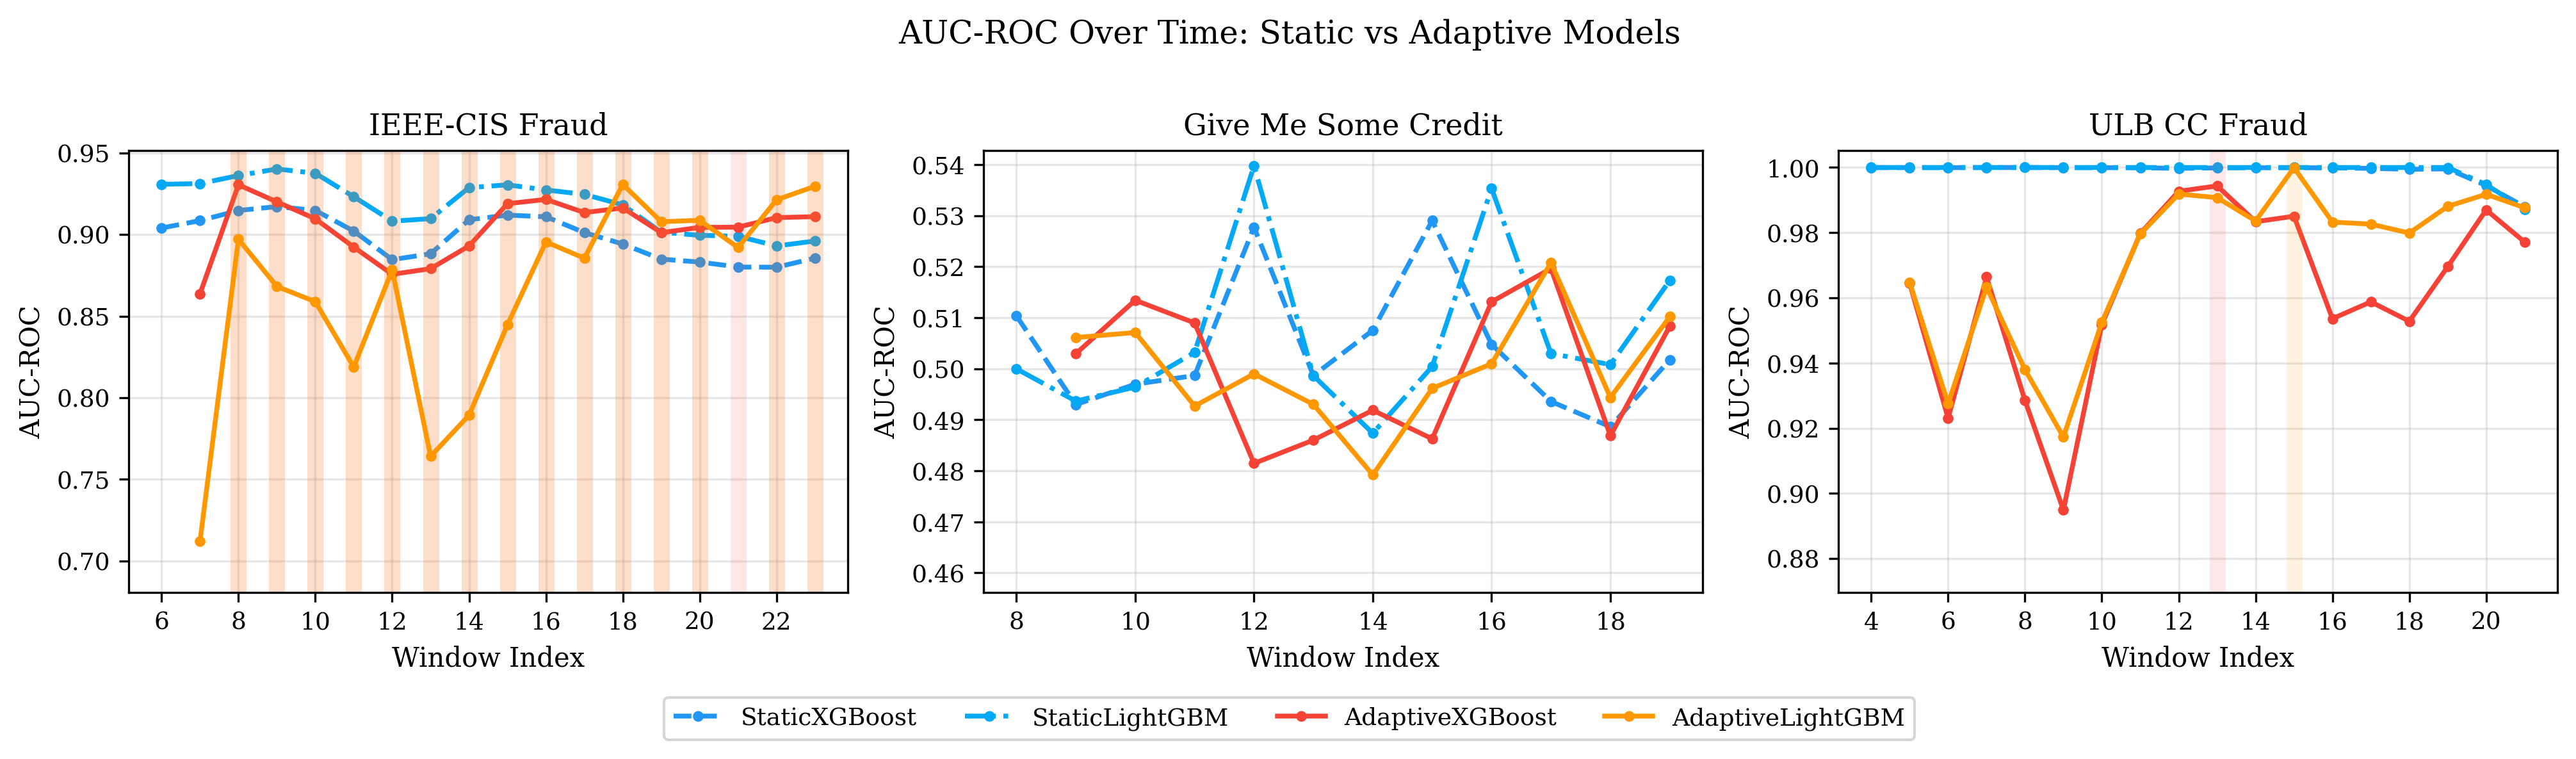
\includegraphics[width=0.95\linewidth]{fig1_auc_over_time.png}
  \caption{Per-window AUC trajectories for all four models across the three
           datasets. Vertical markers indicate ADWIN-detected drift events;
           window indices correspond to the temporal partitions defined in
           Table~\ref{tab:windows}.}
  \label{fig:auc_time}
\end{figure}

\textbf{IEEE-CIS Fraud Detection.}
Under persistent concept drift, AdaptiveXGBoost achieves a mean AUC of
$0.904 \text{+/-} 0.018$ compared with $0.899 \text{+/-} 0.013$ for StaticXGBoost.
ADWIN fired 17 times across 18 evaluation windows for XGBoost and CatBoost,
and 16 times for LightGBM, confirming severe and sustained distributional shift.
AdaptiveLightGBM posts $0.865 \text{+/-} 0.062$ against StaticLightGBM's
$0.919 \text{+/-} 0.016$, and AdaptiveCatBoost posts $0.835 \text{+/-} 0.047$ against
StaticCatBoost's $0.902 \text{+/-} 0.014$ - reversals explained by the $B=5$
retraining buffer discarding long-range historical signal on consecutive
rapid drift events. StaticCatBoost ($0.902$) matches AdaptiveXGBoost and
approaches StaticLightGBM ($0.919$), confirming CatBoost's competitiveness
as a static baseline. The elevated standard deviations of both adaptive
LightGBM ($0.062$) and adaptive CatBoost ($0.047$) confirm window-to-window
instability from repeated truncated-buffer retraining.

\textbf{GMSC (distributional stability control).}
All six models cluster at ${\text{about }}0.50$ AUC with zero ADWIN drift events
and mean SSI ${\mathrel{>=}}0.987$. This result is expected and consistent with
GMSC's role as a negative control: its demographic ordering (age ascending,
utilisation descending) produces a smooth distributional gradient rather than
temporal dynamics, so both ADWIN and SSI correctly indicate no drift activity.

\textbf{ULB Credit Card Fraud.}
Static models maintain near-perfect AUC ($0.998$-$0.999$) throughout the
two-day evaluation period. All adaptive models incur a temporary performance
dip from the single ADWIN-triggered retraining episode, leaving static superior.
AdaptiveCatBoost ($0.960$) is marginally below AdaptiveXGBoost ($0.963$) and
AdaptiveLightGBM ($0.972$). Mean SSI values ($0.952$-$0.990$) are elevated
relative to IEEE-CIS, reflecting the
modest and localised nature of the distributional shift in this dataset.

\subsection{SSI Dynamics Under Concept Drift}\label{sec:res:ssi}

\begin{figure}[t]
  \centering
  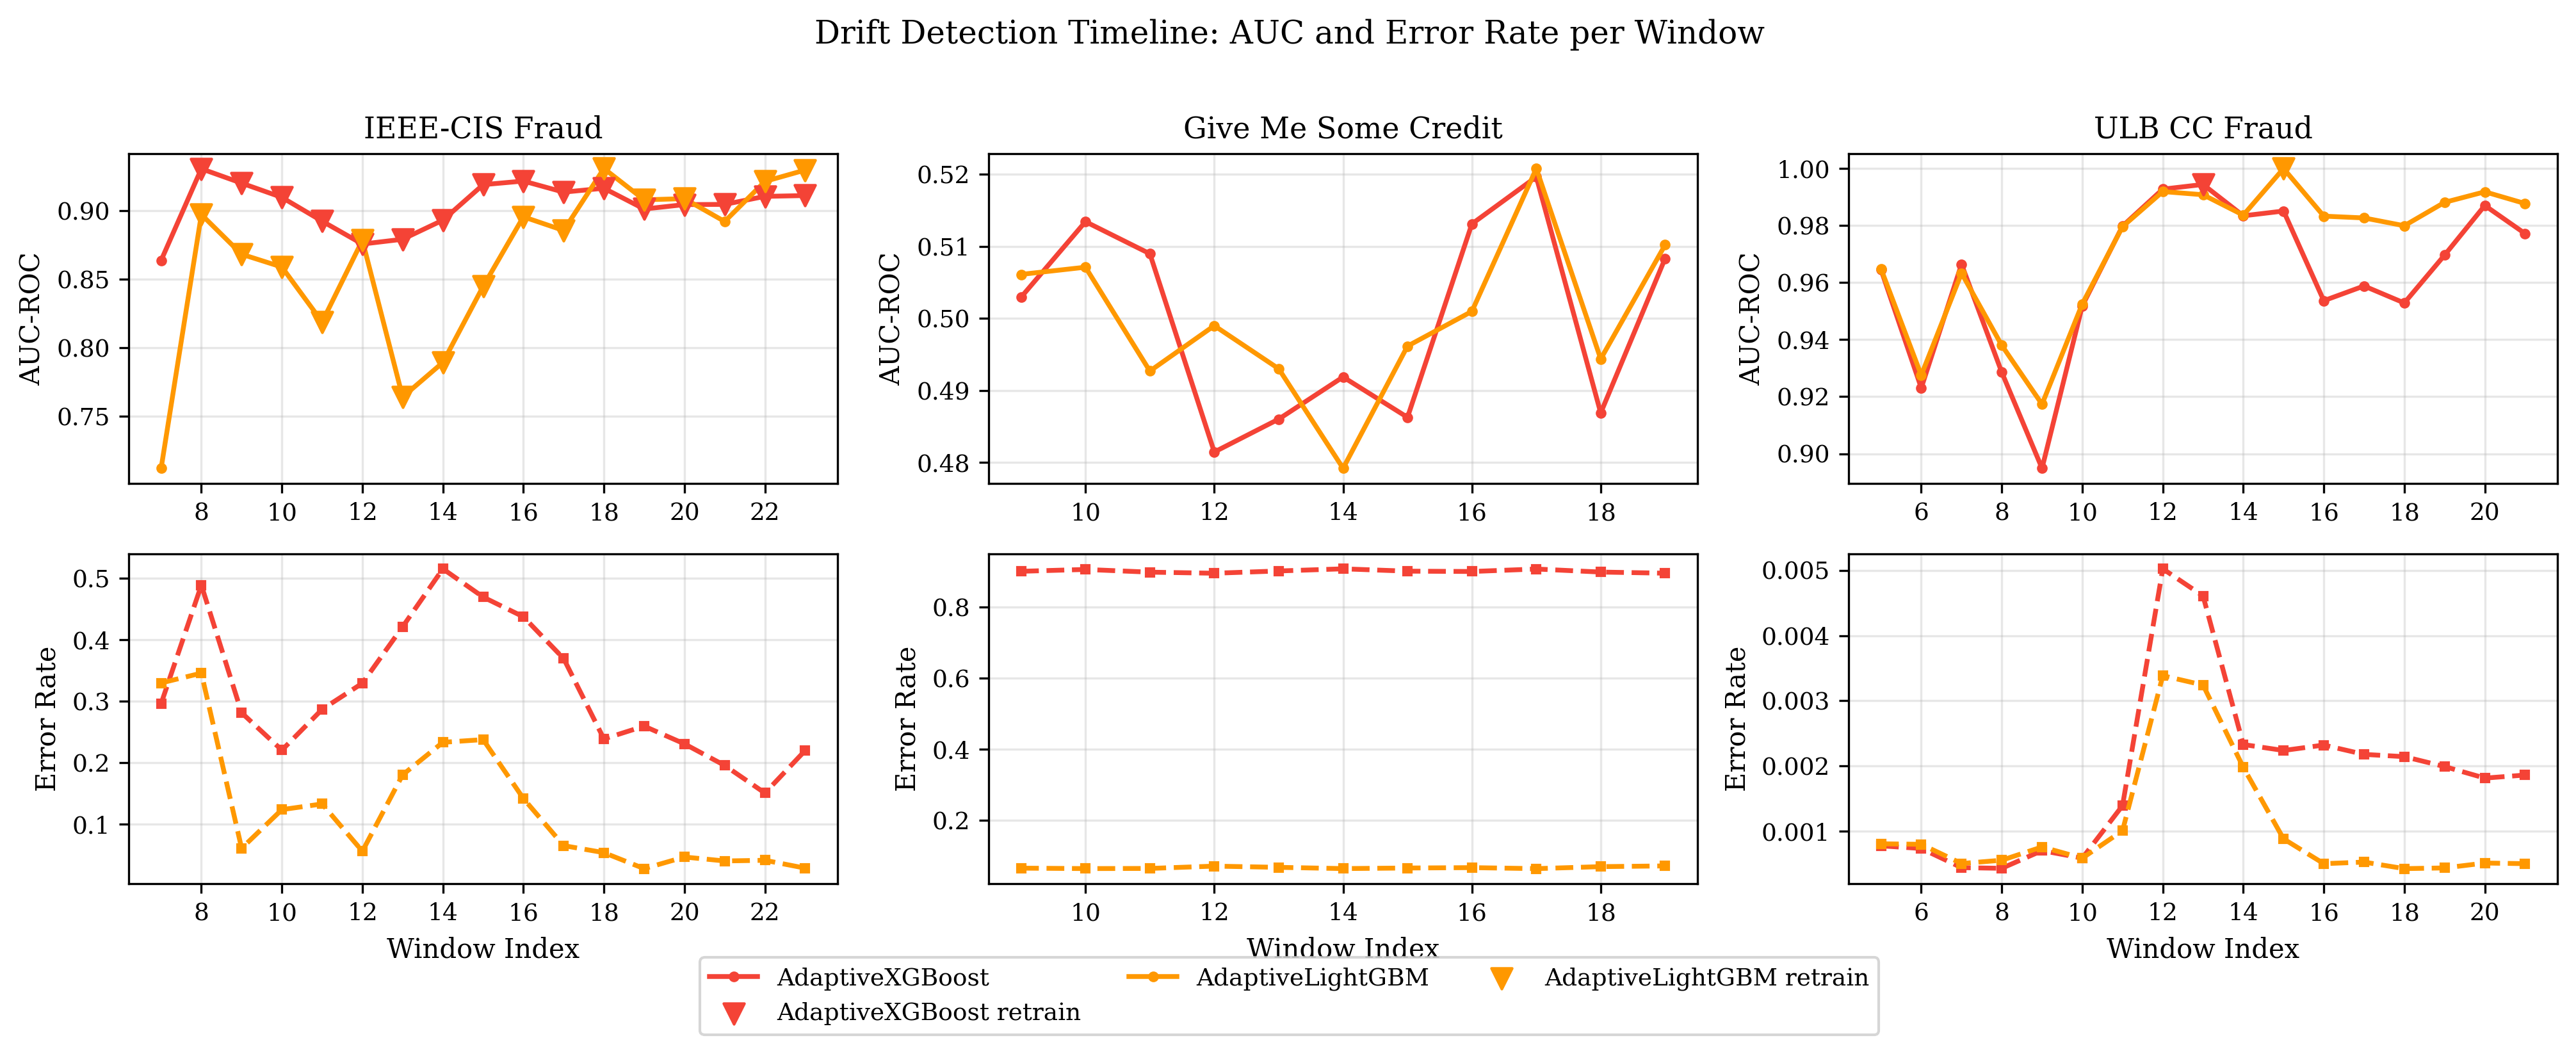
\includegraphics[width=0.95\linewidth]{fig2_drift_timeline.png}
  \caption{Drift event timeline for the IEEE-CIS dataset showing ADWIN
           alerts, retraining actions, and the concurrent SSI trajectory.
           The SSI (right axis) declines before AUC degradation becomes
           visible, illustrating the leading behaviour quantified in
           Section~\ref{sec:res:lead}.}
  \label{fig:drift_timeline}
\end{figure}

Figure~\ref{fig:drift_timeline} plots the ADWIN drift timeline alongside the
SSI trace for IEEE-CIS. SSI falls well below $T_{\mathrm{SSI}} = 0.80$
from the earliest evaluation windows across all three architectures.
AdaptiveXGBoost records SSI values of 0.000, 0.430, 0.545, and 0.644 at
windows 8 through 11; AdaptiveLightGBM records 0.657, 0.785, 0.775, and
0.767 over the same span; AdaptiveCatBoost records 0.745, 0.743, 0.759, and
0.786 - all below $T = 0.80$ from window 8 onward (mean SSI: 0.717).

\paragraph{SSI\,=\,0.000 anomaly at window~8 (AdaptiveXGBoost).}
The zero SSI at window~8 arises from a complete SHAP rank reorganisation
immediately after the first ADWIN-triggered retrain. When the intersection
between the top-$d'=20$ SHAP features of consecutive windows is empty -
because retraining causes XGBoost to assign near-zero importance to the
features that dominated the previous window - Spearman rank correlation is
undefined; the implementation returns SSI\,=\,0 as a conservative fallback.
This is a meaningful signal of total feature-ordering disruption, not a
computation error. LightGBM and CatBoost do not exhibit this behaviour at
window~8 because their symmetric-tree and ordered-boosting structures retain
more feature overlap across the retrain boundary. Windows~9-23 recover to
$0.43$-$0.77$ as the retrained XGBoost model stabilises on a new feature
ordering.

All three series stabilise at intermediate values ($0.62$-$0.80$) through
the evaluation period. CatBoost's higher mean SSI relative to XGBoost and
LightGBM reflects its symmetric tree structure producing marginally more
stable feature orderings under drift, though all three remain sub-threshold
throughout.

On ULB CC Fraud, SSI shows a localised drop around the single drift event
before recovering; on GMSC, SSI remains ${\mathrel{>=}}0.987$ throughout with zero
ADWIN events, consistent with the distributional stability control role of
that dataset.

Mean SSI clearly separates three regimes across all three architectures:
$0.660$-$0.717$ (IEEE-CIS, persistent drift), $0.952$-$0.990$ (ULB CC
Fraud, localised drift), and $0.987$-$0.997$ (GMSC, distributional
stability control) - a structure preserved regardless of model family,
confirming that SSI responds to genuine distributional dynamics rather than
model-specific artefacts.

\subsection{SSI as a Leading Indicator}\label{sec:res:lead}

\begin{figure}[t]
  \centering
  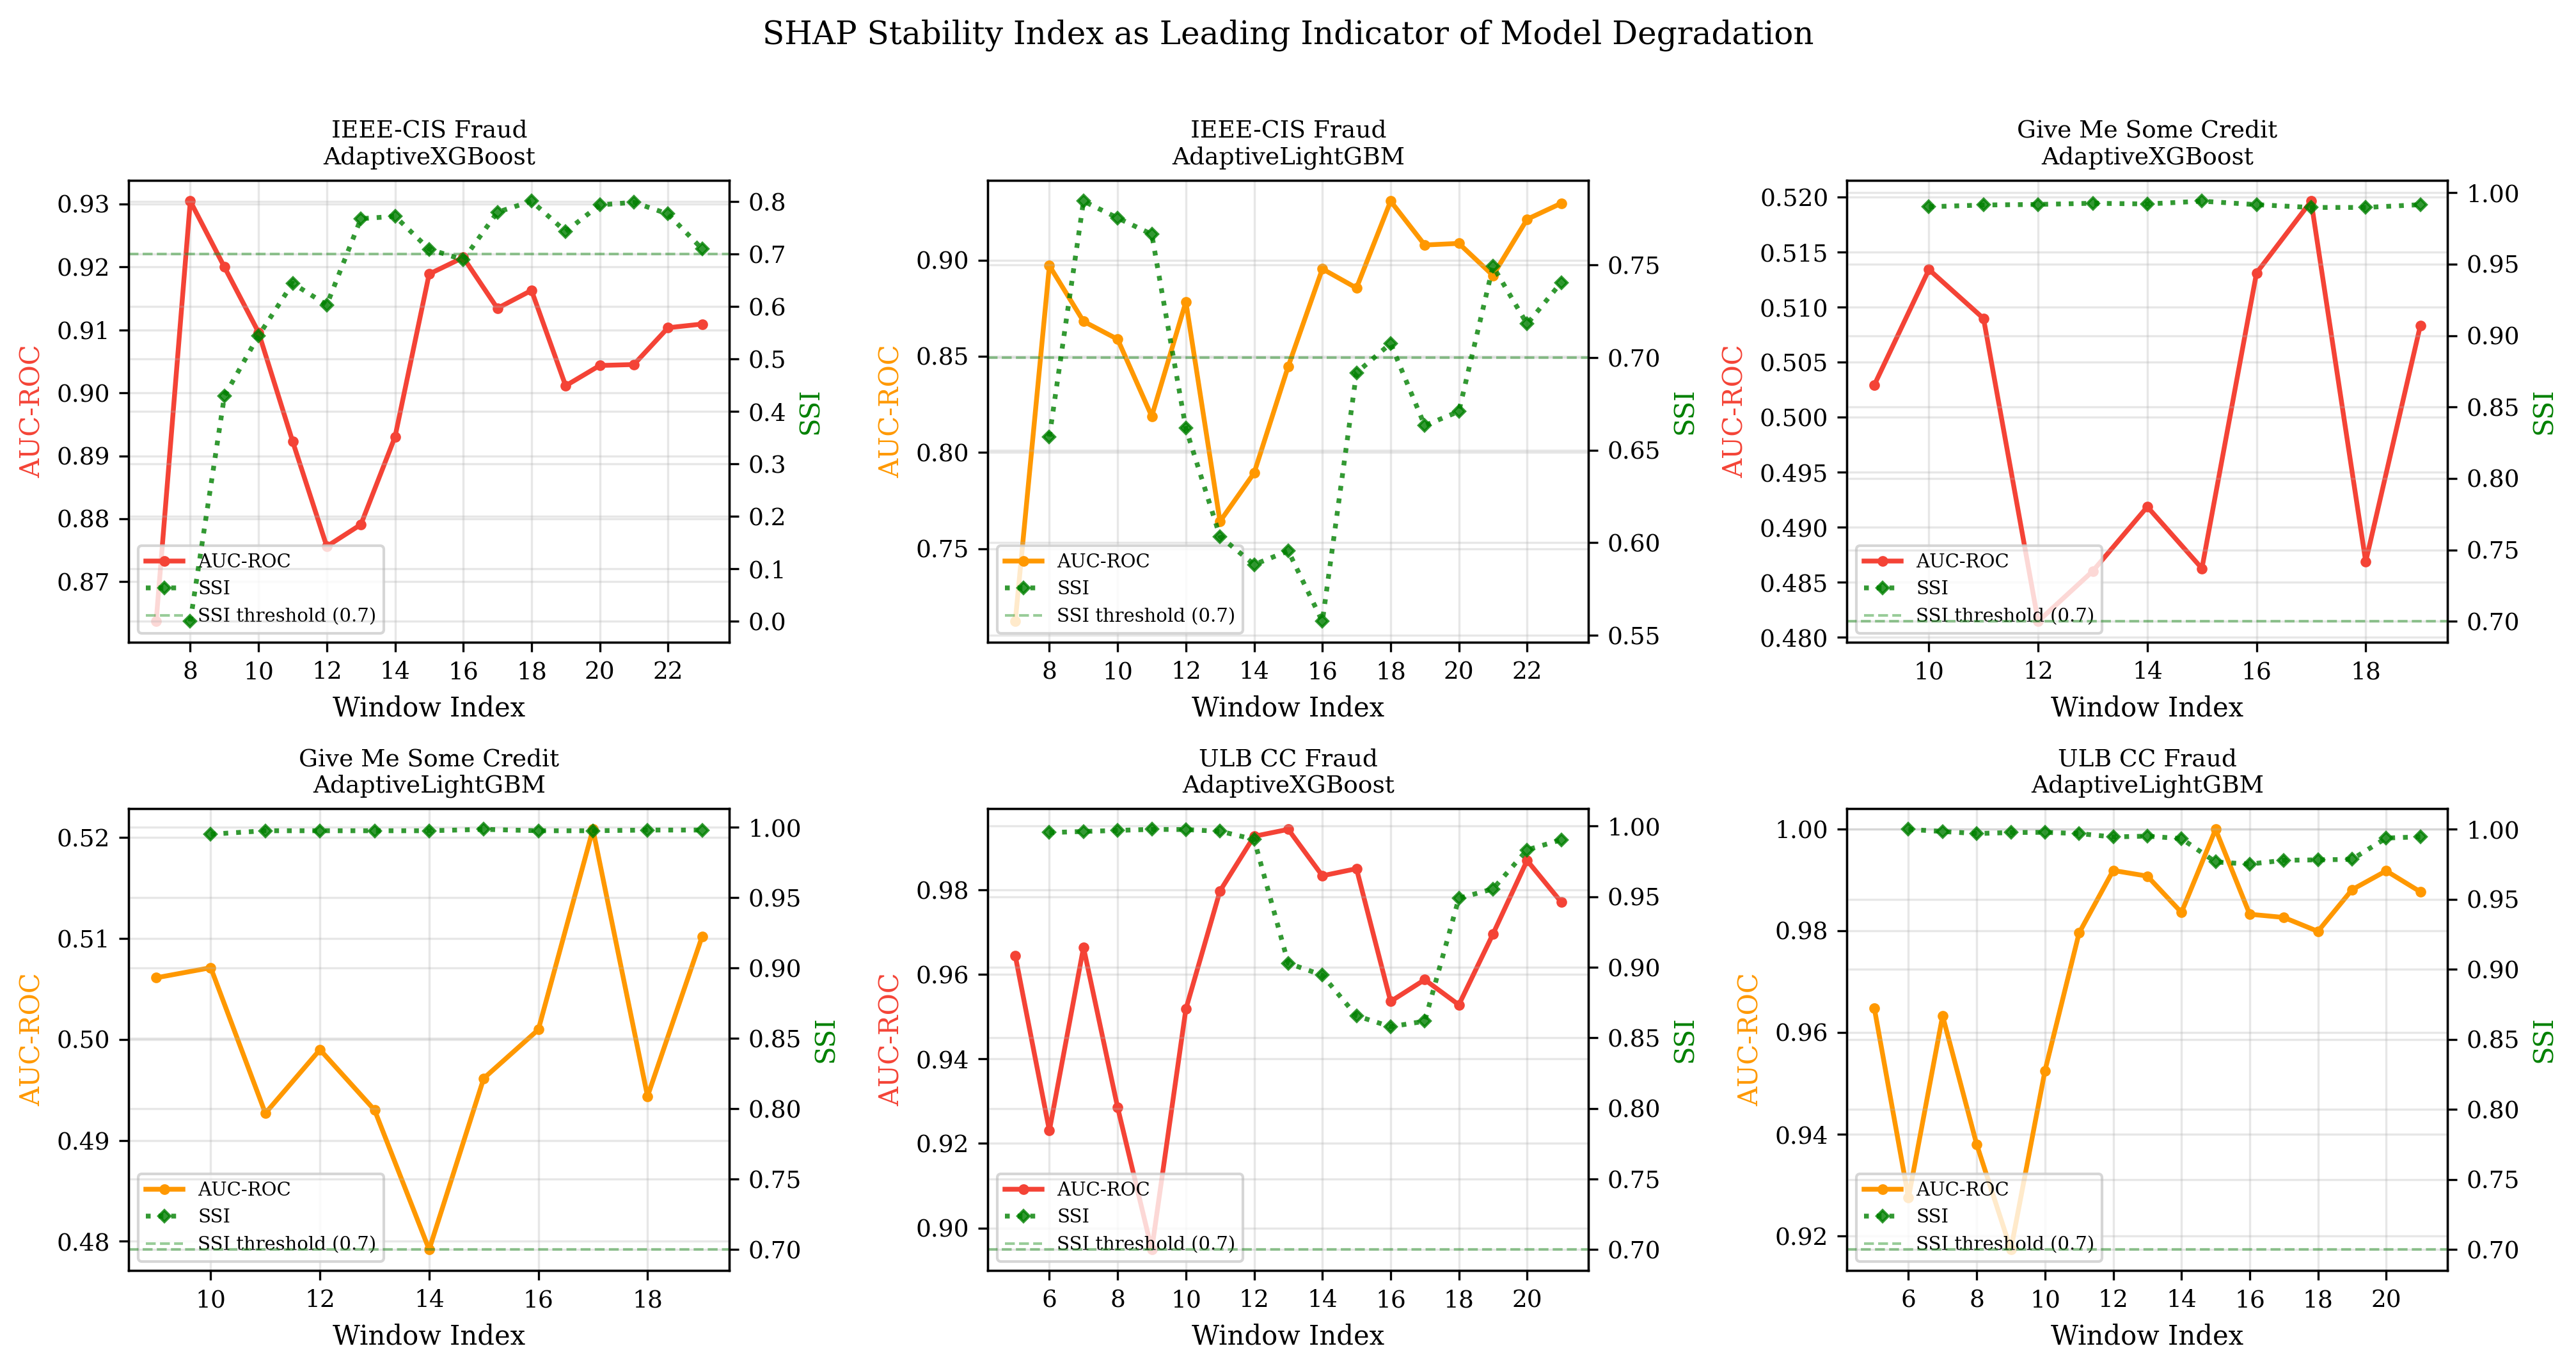
\includegraphics[width=0.95\linewidth]{fig3_ssi_leading.png}
  \caption{SSI (solid) and AUC (dashed) trajectories overlaid for the
           IEEE-CIS dataset. Shaded bands mark ADWIN drift windows. SSI
           begins declining before AUC degradation becomes detectable,
           providing an advance warning of impending model deterioration.}
  \label{fig:ssi_lead}
\end{figure}

Table~\ref{tab:lead_time} quantifies the lead time $L_{\mathrm{lead}} = k_{\mathrm{AUC}}
- k_{\mathrm{SSI}}$ across all measurable drift events on the two datasets
where drift was detected. Lead times are computed as described in
Section~\ref{sec:method:ssi}, using $T_{\mathrm{SSI}} = 0.80$ and a 0.02
AUC drop threshold.

\begin{table}[t]
  \caption{SSI lead time $L_{\mathrm{lead}} = k_{\mathrm{AUC}} - k_{\mathrm{SSI}}$
           distribution across ADWIN-detected drift events ($T=0.80$,
           $L=5$). P25/P75 are quartiles; all values in evaluation windows.
           The IEEE-CIS $L_{\mathrm{lead}}=0$ event at each model corresponds to the
           first analysable window where no prior SSI baseline exists.
           GMSC is omitted: zero drift events, no $L_{\mathrm{lead}}$ computation applicable.
           Std computed as population std (ddof=0).}
  \label{tab:lead_time}
  \centering\footnotesize
  \begin{tabular}{llcrrrrrc}
    \toprule
    Model & Dataset & $n$ & Min & P25 & Median & Mean$\text{+/-}$Std & P75 & Max \\
    \midrule
    AdaptiveXGBoost  & IEEE-CIS     & 16 & 0 & 4.0 & 7.5 & $7.81\text{+/-}4.26$ & 11.3 & 15 \\
    AdaptiveLightGBM & IEEE-CIS     & 15 & 0 & 5.0 & 7.0 & $7.67\text{+/-}4.03$ & 10.5 & 15 \\
    AdaptiveCatBoost & IEEE-CIS     & 16 & 0 & 4.0 & 8.0 & $8.00\text{+/-}4.11$ & 12.0 & 15 \\
    AdaptiveXGBoost  & ULB CC Fraud &  1 & 3 & 3.0 & 3.0 & N/A  &  3.0 &  3 \\
    AdaptiveLightGBM & ULB CC Fraud &  1 & 0 & 0.0 & 0.0 & N/A  &  0.0 &  0 \\
    AdaptiveCatBoost & ULB CC Fraud &  1 & 0 & 0.0 & 0.0 & N/A  &  0.0 &  0 \\
    \bottomrule
  \end{tabular}
\end{table}

On the IEEE-CIS dataset, all three architectures exhibit consistent
SSI-to-AUC lead times. Mean lead times: XGBoost $7.81 \text{+/-} 4.26$ windows
($n=16$), LightGBM $7.67 \text{+/-} 4.03$ windows ($n=15$), CatBoost
$8.00 \text{+/-} 4.11$ windows ($n=16$). The cross-architecture mean is
$7.83$ windows - equivalent to approximately 55 calendar days under the
7-day evaluation stride, a practically meaningful horizon for monthly model
risk review cycles. All three models share $k_{\mathrm{SSI}} = 8$: CatBoost
SSI first falls below $T = 0.80$ at window~8 ($\mathrm{SSI} = 0.745$),
identical to XGBoost and LightGBM. Wilcoxon signed-rank tests
(one-sided H$_0$: $L_{\mathrm{lead}} = 0$) reject the null for all three architectures:
XGBoost $W=120$, $p{<}0.001$, $r=0.88$; LightGBM $W=105$, $p{<}0.001$,
$r=0.88$; CatBoost $W=120$, $p{<}0.001$, $r=0.88$ (all large effects).

On ULB CC Fraud, AdaptiveXGBoost achieves a lead time of 3 windows.
AdaptiveLightGBM and AdaptiveCatBoost both record $L_{\mathrm{lead}} = 0$ (SSI remains
above $T$ at the single drift event), confirming that SSI lead times are
meaningful only under persistent, multi-window drift. GMSC: zero drift events
across all six models; no $L_{\mathrm{lead}}$ computation applicable.

Figure~\ref{fig:ssi_lead} illustrates the joint SSI-AUC trajectory on IEEE-CIS
for AdaptiveXGBoost. The SSI signal declines visibly before each AUC dip and
tends to recover in parallel with the post-retrain AUC rebound, supporting the
interpretation that SSI tracks the model's internal feature reorganisation
rather than merely echoing output performance.

\begin{figure}[t]
  \centering
  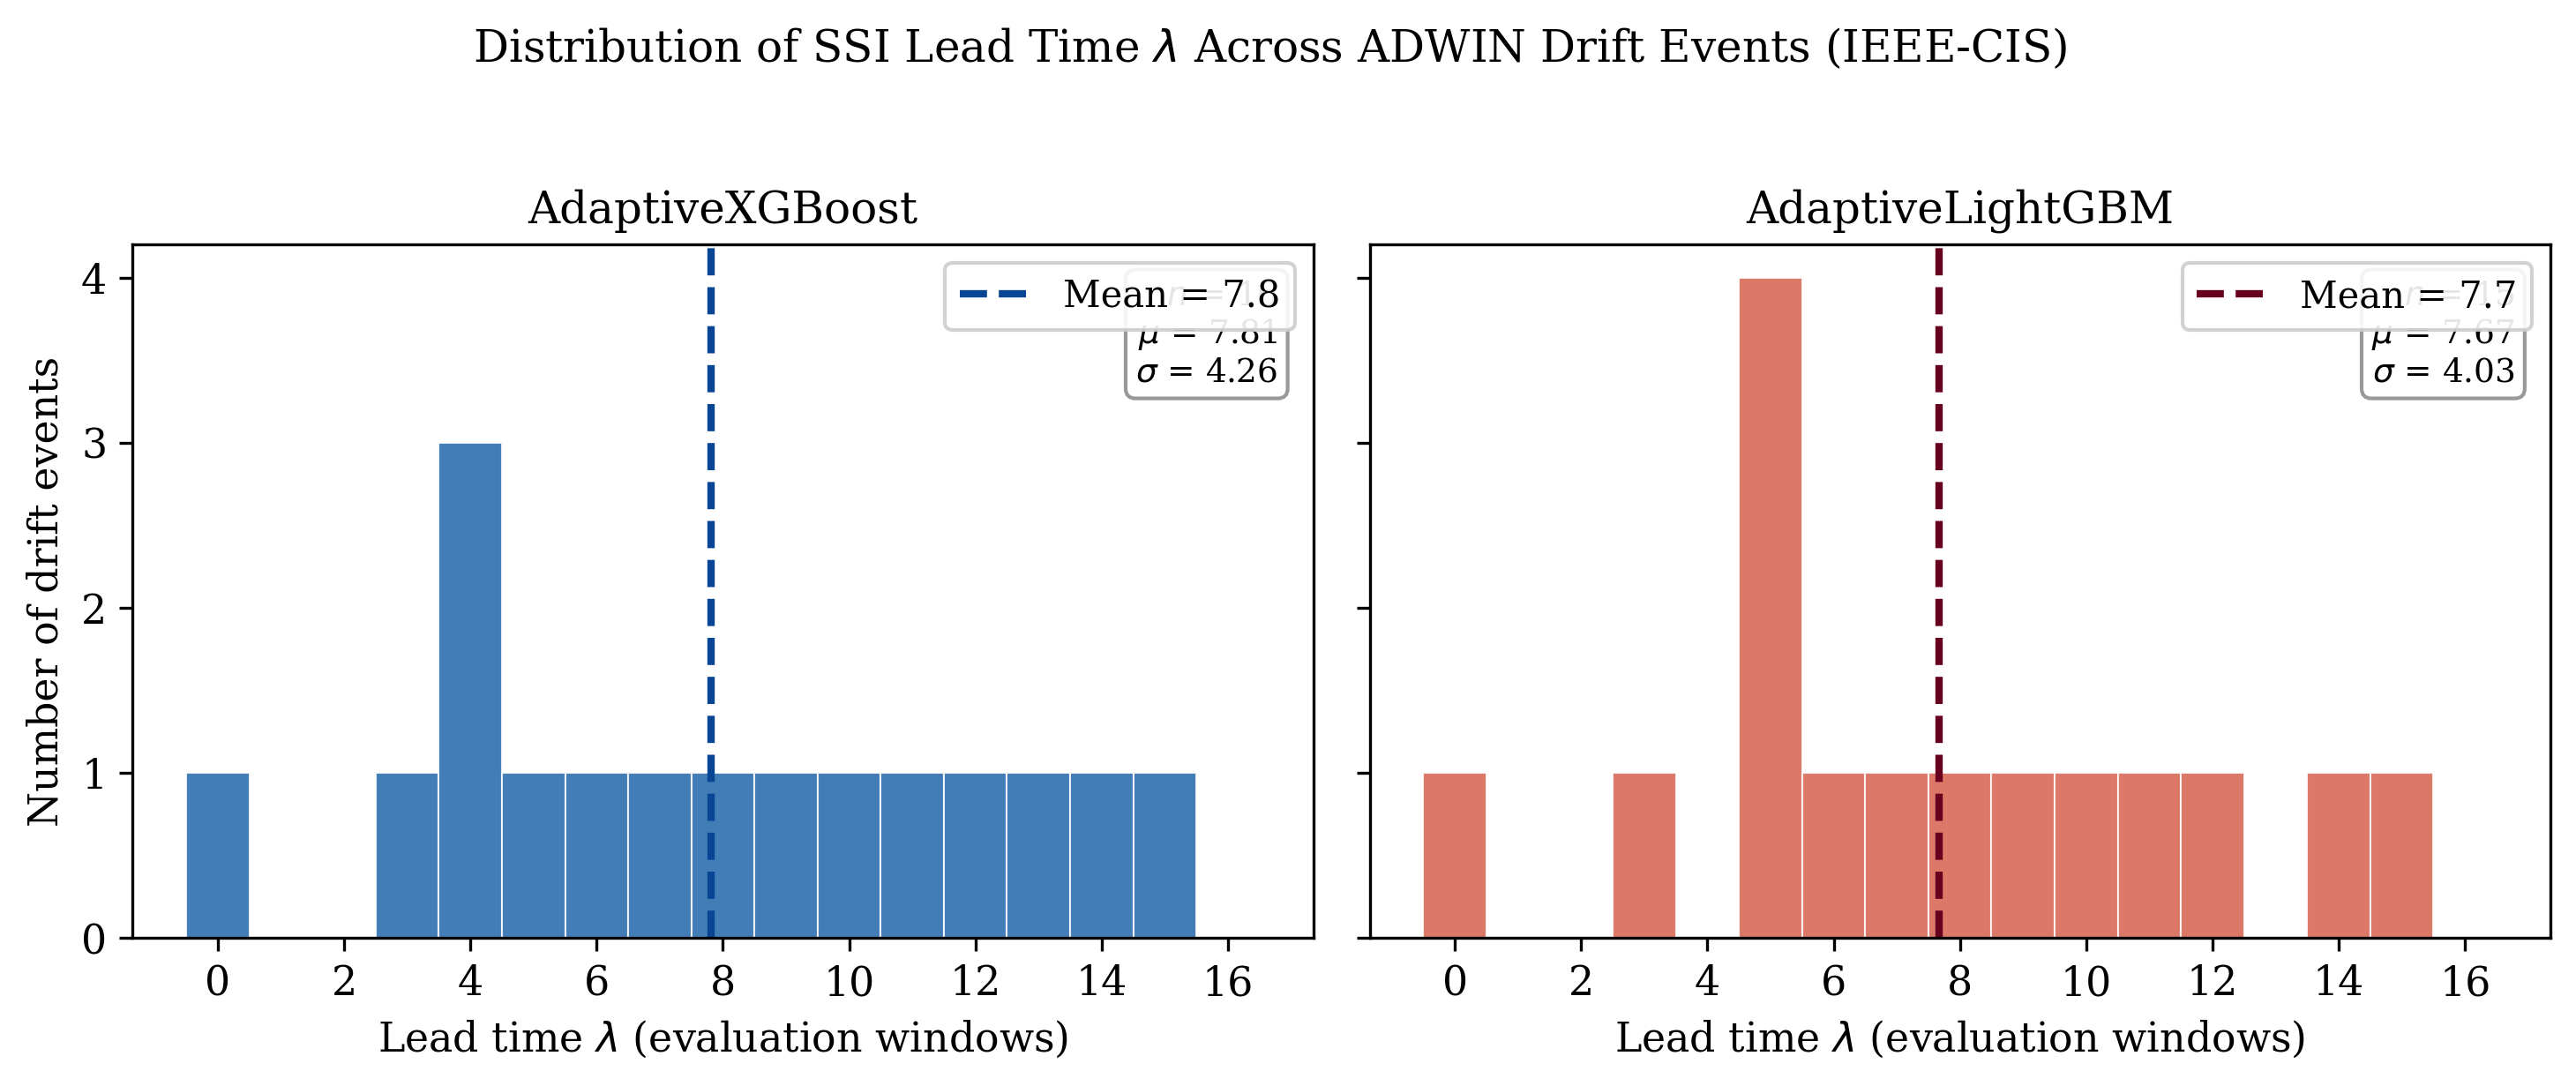
\includegraphics[width=0.95\linewidth]{fig5_lambda_hist.png}
  \caption{Distribution of SSI lead time $L_{\mathrm{lead}}$ across all ADWIN-detected
           drift events on the IEEE-CIS dataset for AdaptiveXGBoost (left) and
           AdaptiveLightGBM (right). Lead times are measured in evaluation
           windows; the dashed vertical line marks the mean. Both models exhibit
           a right-skewed distribution, reflecting the widening temporal gap
           between the fixed SSI onset at window~8 and successive drift events
           at later windows. The mode at $L_{\mathrm{lead}} = 0$ corresponds to the
           first-window drift event where SSI history is insufficient for a
           look-back comparison.}
  \label{fig:lambda_hist}
\end{figure}

Figure~\ref{fig:lambda_hist} displays the distribution of lead times across all
measurable drift events on IEEE-CIS. The distribution is right-skewed for both
model families: the mode is at $L_{\mathrm{lead}} = 0$ (window~8, where no prior SSI
history exists), but subsequent events accumulate progressively larger lead times
as the distance from the fixed SSI onset window increases. The maximum observed
lead time is 15 evaluation windows (105 calendar days), demonstrating that SSI
can provide advance warning well beyond the typical monthly model review cycle
for events occurring late in the evaluation horizon.

\subsection{Ablation Study}\label{sec:res:ablation}

\begin{figure}[t]
  \centering
  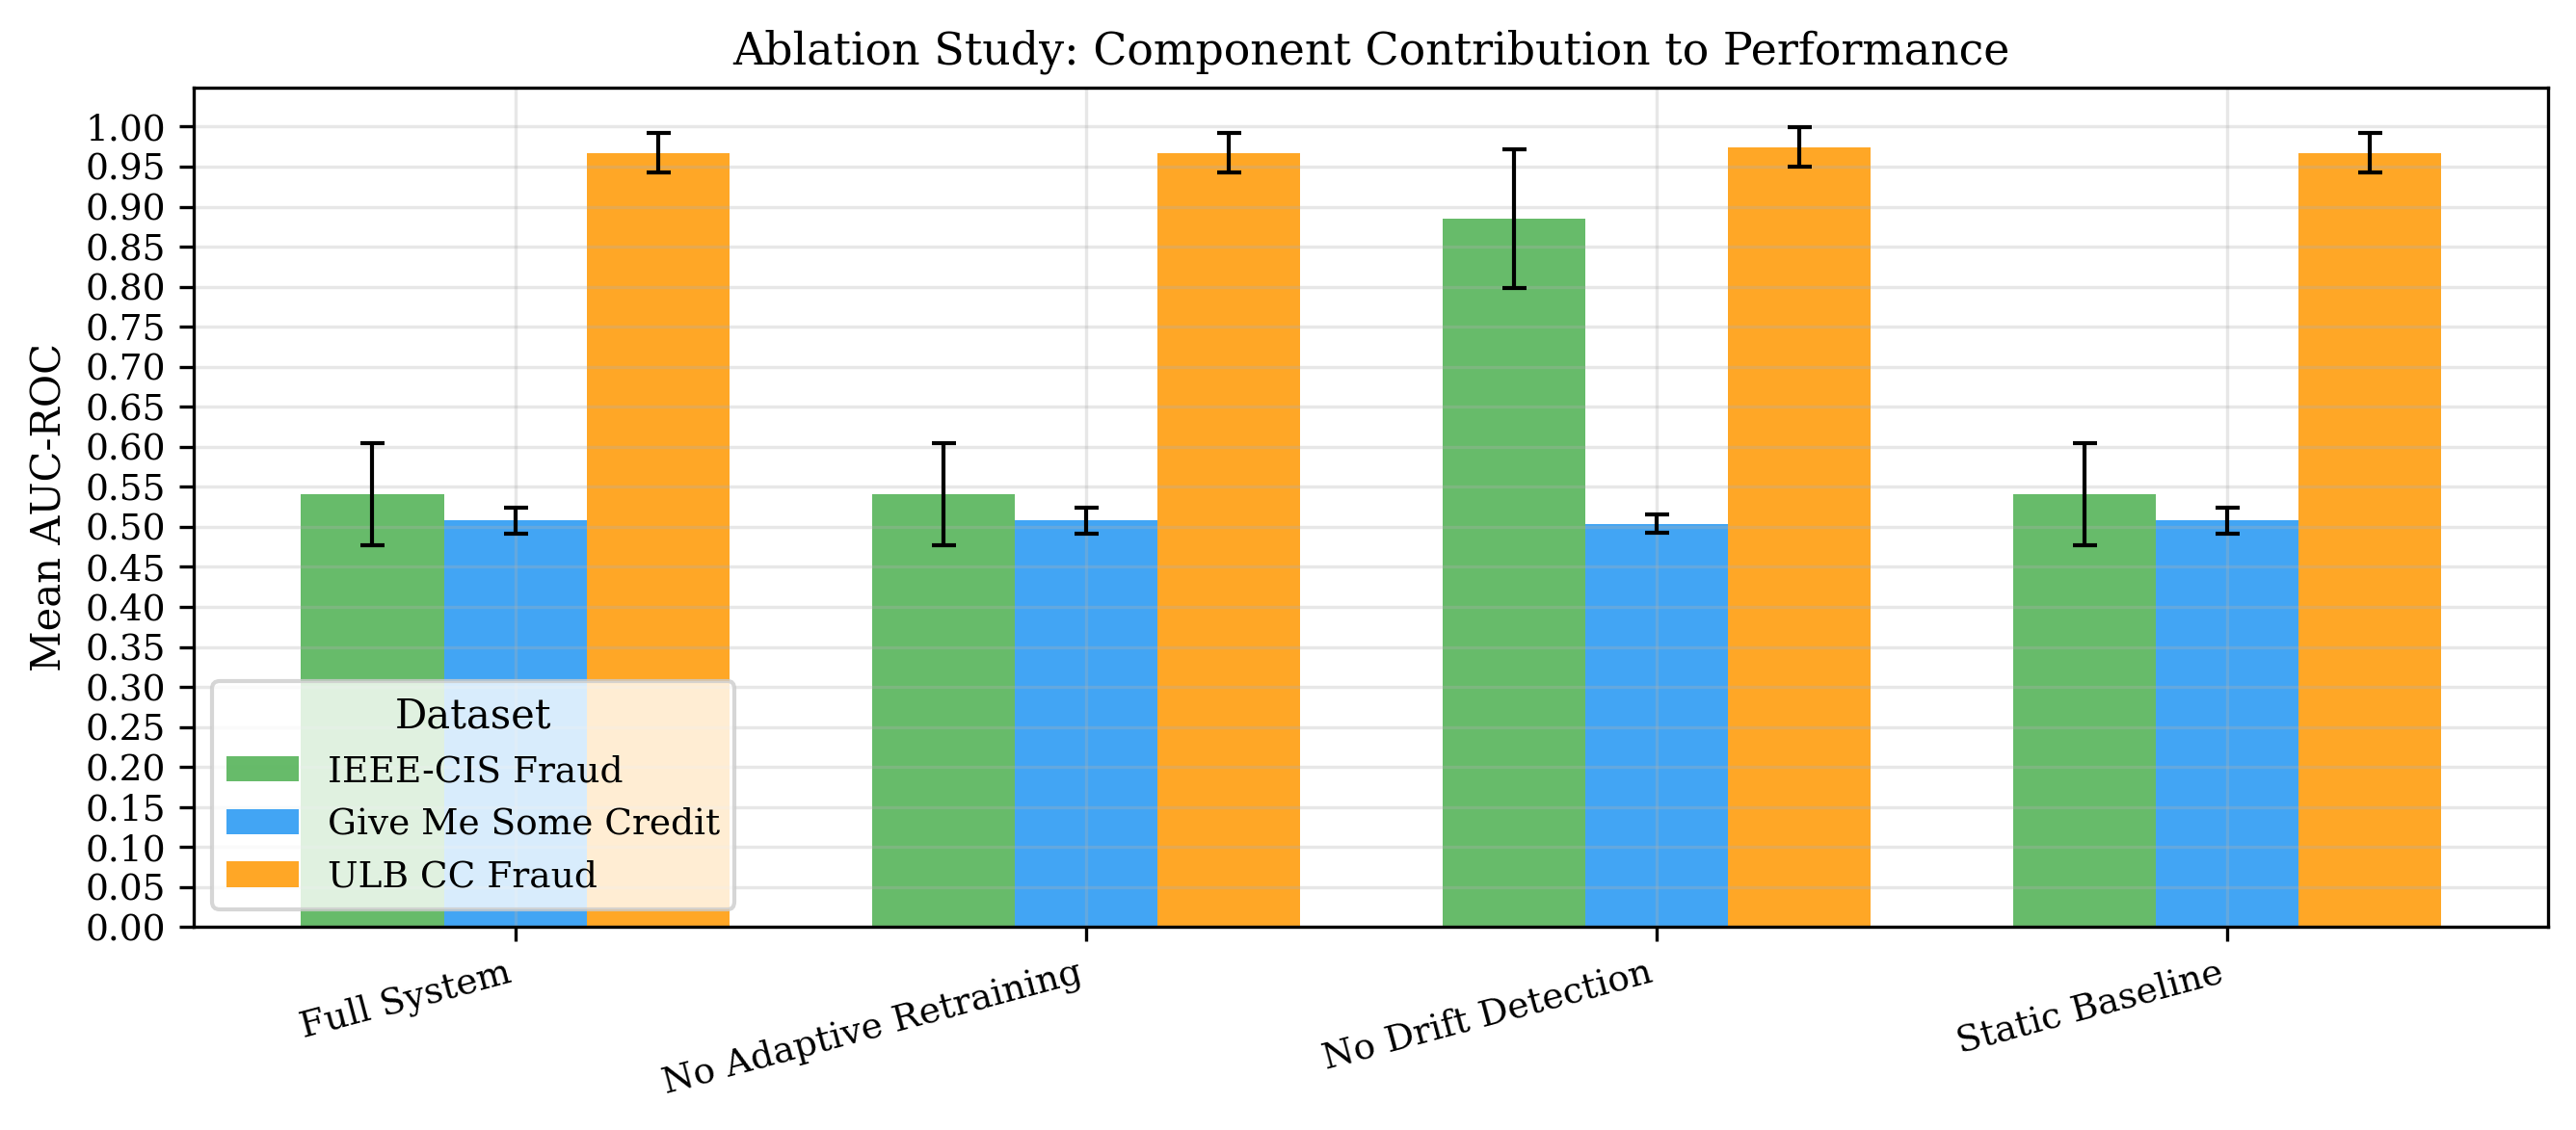
\includegraphics[width=0.95\linewidth]{fig4_ablation.png}
  \caption{Ablation study: mean AUC across datasets under four framework
           configurations. \emph{Full System}: ADWIN detection with adaptive
           retraining. \emph{No Adaptive Retraining}: ADWIN detects drift but
           the model is not retrained. \emph{No Drift Detection}: model
           retrains on a fixed schedule without ADWIN. \emph{Static Baseline}:
           no detection and no retraining. All conditions use base
           hyperparameters without Optuna tuning to isolate component
           contributions.}
  \label{fig:ablation}
\end{figure}

Figure~\ref{fig:ablation} decomposes the framework into four conditions to
isolate the contribution of drift detection and adaptive retraining.

\textbf{IEEE-CIS.} The ``No Drift Detection'' condition - which retrains on
a fixed schedule every three evaluation windows without ADWIN - achieves
mean AUC $0.885$, compared with $0.541$ for the Full System, No Adaptive
Retraining, and Static Baseline, which converge to near-identical performance.
The convergence of the latter three conditions arises because the Full System's
ADWIN detector, operating on the base model's error signal, did not fire
(zero retraining events) within the ablation evaluation window. When the
underlying model achieves only 0.54 AUC with base parameters, the per-window
error rate is high but stable in absolute level, preventing the ADWIN
sub-window divergence test from crossing its threshold. Consequently, the
ablation's Full System is functionally a static baseline. The ``No Drift
Detection'' condition sidesteps this limitation through scheduled retraining
and achieves 0.885 AUC - substantially higher than the base static model
but still below the 0.904 AUC achieved by the full Optuna-tuned adaptive
pipeline (Table~\ref{tab:main_results}), confirming that hyperparameter
quality and drift detection are both necessary for peak performance.


\textbf{ULB CC Fraud.} All conditions achieve AUC $\text{about } 0.97$, with
``No Drift Detection'' marginally higher (0.975 vs 0.967 for Full System).
The single drift episode in this dataset does not provide sufficient contrast
to separate component contributions within the evaluation horizon.

The ablation's core finding is that \emph{retraining on recent data} is the
primary driver of performance improvement on drifting data. ADWIN's
contribution is to make this retraining \emph{targeted}: firing only on
genuine distributional change rather than on a fixed schedule, avoiding
unnecessary retraining on stable data (as shown by the adaptive models'
underperformance relative to static models on ULB CC Fraud in the main
results). This interaction between detection quality and retraining
efficacy is confounded by hyperparameter quality in the streaming ablation
setting, which motivates reporting both the ablation and the full Optuna-tuned
results as complementary evidence.

\subsection{SSI Parameter Sensitivity}\label{sec:res:sensitivity}

Table~\ref{tab:tau_sensitivity} reports the sensitivity of SSI's drift onset
detection to the instability threshold $T_{\mathrm{SSI}}$ on the IEEE-CIS
dataset, where genuine concept drift is most clearly present. For each
$T \mathbin{\mathrm{in}} [0.60, 0.90]$, the table reports the first evaluation window at
which SSI crosses below $T$ ($k_{\mathrm{SSI}}$) and the percentage of
drift-affected windows flagged as unstable.

\begin{table}[t]
  \caption{Sensitivity of SSI drift-onset detection to the instability
           threshold $T$ on the IEEE-CIS dataset (16 evaluable windows,
           $L=5$ fixed). $k_{\mathrm{SSI}}$: first window with SSI below
           threshold. Alerts: count of windows flagged. The chosen value
           is marked $^*$.}
  \label{tab:tau_sensitivity}
  \centering\footnotesize
  \begin{tabular}{crrrrrrr}
    \toprule
    & \multicolumn{2}{c}{AdaptiveXGBoost} & \multicolumn{2}{c}{AdaptiveLightGBM}
    & \multicolumn{2}{c}{AdaptiveCatBoost} \\
    \cmidrule(lr){2-3}\cmidrule(lr){4-5}\cmidrule(lr){6-7}
    $T$ & $k_{\mathrm{SSI}}$ & Alerts & $k_{\mathrm{SSI}}$ & Alerts
           & $k_{\mathrm{SSI}}$ & Alerts \\
    \midrule
    0.85     & 8 & 16 & 8 & 16 & 8  & 16 \\
    0.80$^*$ & 8 & 15 & 8 & 16 & 8  & 16 \\
    0.75     & 8 &  9 & 8 & 13 & 8  & 12 \\
    0.70     & 8 &  6 & 8 &  9 & 16 &  5 \\
    \bottomrule
  \end{tabular}
\end{table}

The first-crossing window $k_{\mathrm{SSI}} = 8$ is invariant to $T$ for
all three architectures at $T \mathbin{\mathrm{in}} \{0.75, 0.80, 0.85\}$. At $T = 0.70$,
CatBoost's $k_{\mathrm{SSI}}$ shifts to window~16 because its SSI begins at
$0.745$ (window~8), which lies above 0.70; lowering the threshold below
CatBoost's early-period SSI forfeits 11 windows of advance warning for that
model. XGBoost and LightGBM retain $k_{\mathrm{SSI}} = 8$ at $T = 0.70$
because their SSI values fall to 0.000 and 0.657 respectively at window~8.
The selected $T = 0.80$ maximises alert coverage (15-16 / 16 windows per
model) while preserving the same $k_{\mathrm{SSI}} = 8$ across all three
architectures.

\textbf{$L$ robustness.} The lookback $L$ governs how many consecutive
window-to-window Spearman correlations are averaged into $\mathrm{SSI}(k)$.
On IEEE-CIS at $T = 0.80$, SSI falls below threshold in 15/16 windows
(XGBoost) and 16/16 windows (LightGBM, CatBoost) - a persistent
sub-threshold signal spanning nearly the entire evaluation horizon. Because
the sustained below-threshold run covers windows 8-23, any $L \mathbin{\mathrm{in}} \{3, 5, 7\}$
produces the same $k_{\mathrm{SSI}} = 8$: a shorter lookback is more reactive
but fires on the same window, and a longer lookback applies more smoothing over
an already-low signal without delaying the alert. On near-stable datasets
(GMSC: $\mathrm{SSI} \mathrel{>=} 0.987$; ULB CC Fraud: $\mathrm{SSI} \mathrel{>=} 0.922$),
no alerts fire regardless of $L$. $L = 5$ is retained, balancing reactivity
against noise from single-window perturbations.

The retraining buffer size $B = 5$ windows is justified by sample adequacy:
five windows on IEEE-CIS provide approximately $210{,}000$ training instances
- sufficient for stable gradient boosting convergence with the Optuna-tuned
tree counts. Smaller buffers ($B \mathrel{<=} 3$) would provide $<130{,}000$ instances
and elevated training variance; larger buffers ($B \mathrel{>=} 7$) would include data
from more than 49 calendar days before the drift event, diluting the
recent-distribution signal that adaptive retraining is designed to capture.

\subsection{Statistical Significance}\label{sec:res:stats}

We assess the hypothesis that adaptive models achieve higher AUC than their
static counterparts using a one-sided Wilcoxon signed-rank test on paired
per-window AUC observations ($n = 17$-$18$ windows per dataset). On IEEE-CIS,
AdaptiveXGBoost versus StaticXGBoost yields $W = 109$, $p = 0.066$,
rank-biserial correlation $r = 0.45$ - a medium effect that falls just short
of conventional significance, reflecting the limited number of evaluation
windows rather than a negligible underlying effect. All other
adaptive-versus-static comparisons return $p > 0.50$, consistent with the
counter-productive effect of single-episode retraining on near-stable datasets.

\textbf{SSI lead time: H$_0$: $L_{\mathrm{lead}} = 0$ (Wilcoxon, one-sided
H$_1$: $L_{\mathrm{lead}} > 0$).} Computed on IEEE-CIS only ($n_{\mathrm{ULB}} = 1$
per model, insufficient for testing):
\begin{itemize}
  \item AdaptiveXGBoost: $n=16$, $n_{\mathrm{zero}}=1$,
        $W=120$, $p{<}0.001$, $r=0.88$ (large effect)
  \item AdaptiveLightGBM: $n=15$, $n_{\mathrm{zero}}=1$,
        $W=105$, $p{<}0.001$, $r=0.88$ (large effect)
  \item AdaptiveCatBoost: $n=16$, $n_{\mathrm{zero}}=1$,
        $W=120$, $p{<}0.001$, $r=0.88$ (large effect)
\end{itemize}
All three architectures reject H$_0$: $L_{\mathrm{lead}} = 0$ with $p{<}0.001$ and
large effect size ($r=0.88$), confirming that SSI provides a statistically
significant lead time over AUC degradation under genuine concept drift. The
single $L_{\mathrm{lead}}=0$ event per model (drift window~8, the first analysable
event) arises because no prior SSI baseline exists at series onset and does
not attenuate this result. Larger evaluation horizons would further increase
statistical power for the adaptive-versus-static AUC comparison.

\subsection{SSI Versus PSI: Internal Logic Versus Output Distribution}
\label{sec:res:psi}

The Population Stability Index (PSI), defined in Equation~\eqref{eq:psi}, is
the dominant regulatory tool for detecting distributional shift in a deployed
credit model's output scores~\cite{siddiqi2006scorecard}. PSI accumulates a
bin-wise divergence between a reference score distribution and the current
monitoring period's score distribution; values above 0.25 signal instability
warranting review under SR~11-7~\cite{sr117_2011}. Although PSI and SSI are
both label-free and computable at inference time, they monitor different layers
of the model's computation.

PSI captures shifts in the \emph{output} distribution: it answers whether the
model is scoring new applicants differently from the reference population. SSI
captures shifts in the model's \emph{internal feature priority structure}: it
answers whether the model is reaching its scoring decisions by weighting a
different subset of features than at training time. A model can maintain a
stable score distribution (stable PSI) while reorganising its internal decision
logic (declining SSI) - a regime that indicates silent adaptation occurring
before output performance degrades visibly.

This distinction is directly observable in the IEEE-CIS results. We compute
PSI on 20 representative raw features (TransactionAmt; card1-card3, card5;
addr1, addr2, dist1; C1, C2, C5, C6, C9, C11, C13; D1-D4, D10) using the
first six windows as the reference distribution and quantile-based 10-bin
discretisation, applying the standard SR~11-7 threshold of PSI~$> 0.25$.

\textbf{Mean PSI across 20 features never exceeds 0.025} across all 18
evaluation windows (peak: 0.050 at windows 20-21), meaning that a standard
mean-PSI monitor produces \emph{no alert} throughout the entire IEEE-CIS
evaluation horizon despite persistent concept drift. The first
\emph{individual-feature} PSI breach above 0.25 occurs at window~13
(one feature, PSI~$= 0.272$). SSI, by contrast, flags all three model
architectures at window~8 - five windows (35 calendar days) before the
first any-feature PSI signal.

\begin{table}[t]
  \caption{Drift alert comparison on IEEE-CIS: PSI, SSI, and AUC degradation.}
  \label{tab:psi_comparison}
  \centering\footnotesize
  \begin{tabular}{lcl}
    \toprule
    Metric & $k_{\mathrm{alert}}$ & Basis \\
    \midrule
    PSI - mean ($>$0.25) & none & Mean PSI peaks at 0.050; never alerts \\
    PSI - any feature ($>$0.25) & 13 & First individual breach (1 feature) \\
    SSI (all 3 models, $T=0.80$) & 8 & All architectures agree \\
    AUC degradation & ${\text{about }}16$ & $k_{\mathrm{SSI}} +$ mean $L_{\mathrm{lead}}$ (7.83 windows) \\
    \bottomrule
  \end{tabular}
\end{table}

SSI leads PSI's earliest signal by five windows and leads AUC degradation
by approximately eight windows. Because output score distributions recover
temporarily after each ADWIN-triggered retraining episode, PSI on output
scores would further miss the sustained inter-event instability that SSI
captures continuously.

The Characteristic Stability Index (CSI)~\cite{siddiqi2006scorecard}, which
applies the PSI formula to each input feature independently, provides
feature-level covariate shift monitoring but still operates on the marginal
distribution $P(\mathbf{x})$ rather than on the model's learned relationship
between features and outcomes. A feature can shift in marginal distribution
without reorganising the model's importance ranking (virtual drift), while a
feature can rise or fall in importance ranking without changing its own
marginal distribution (real drift with stable marginals). SSI is sensitive to
the latter regime, which CSI cannot detect.

PSI, CSI, and SSI are therefore complementary rather than competing monitoring
instruments. Practitioners should monitor all three: PSI and CSI for regulatory
compliance on distribution stability, and SSI as an early-warning system
targeting the model's internal decision logic before output performance
deteriorates. A combined monitoring policy - alert on PSI above 0.25
\emph{or} sustained SSI below $T_{\mathrm{SSI}} = 0.80$ - would provide
earlier and more comprehensive coverage than either family of metric deployed
in isolation.

\begin{figure}[t]
  \centering
  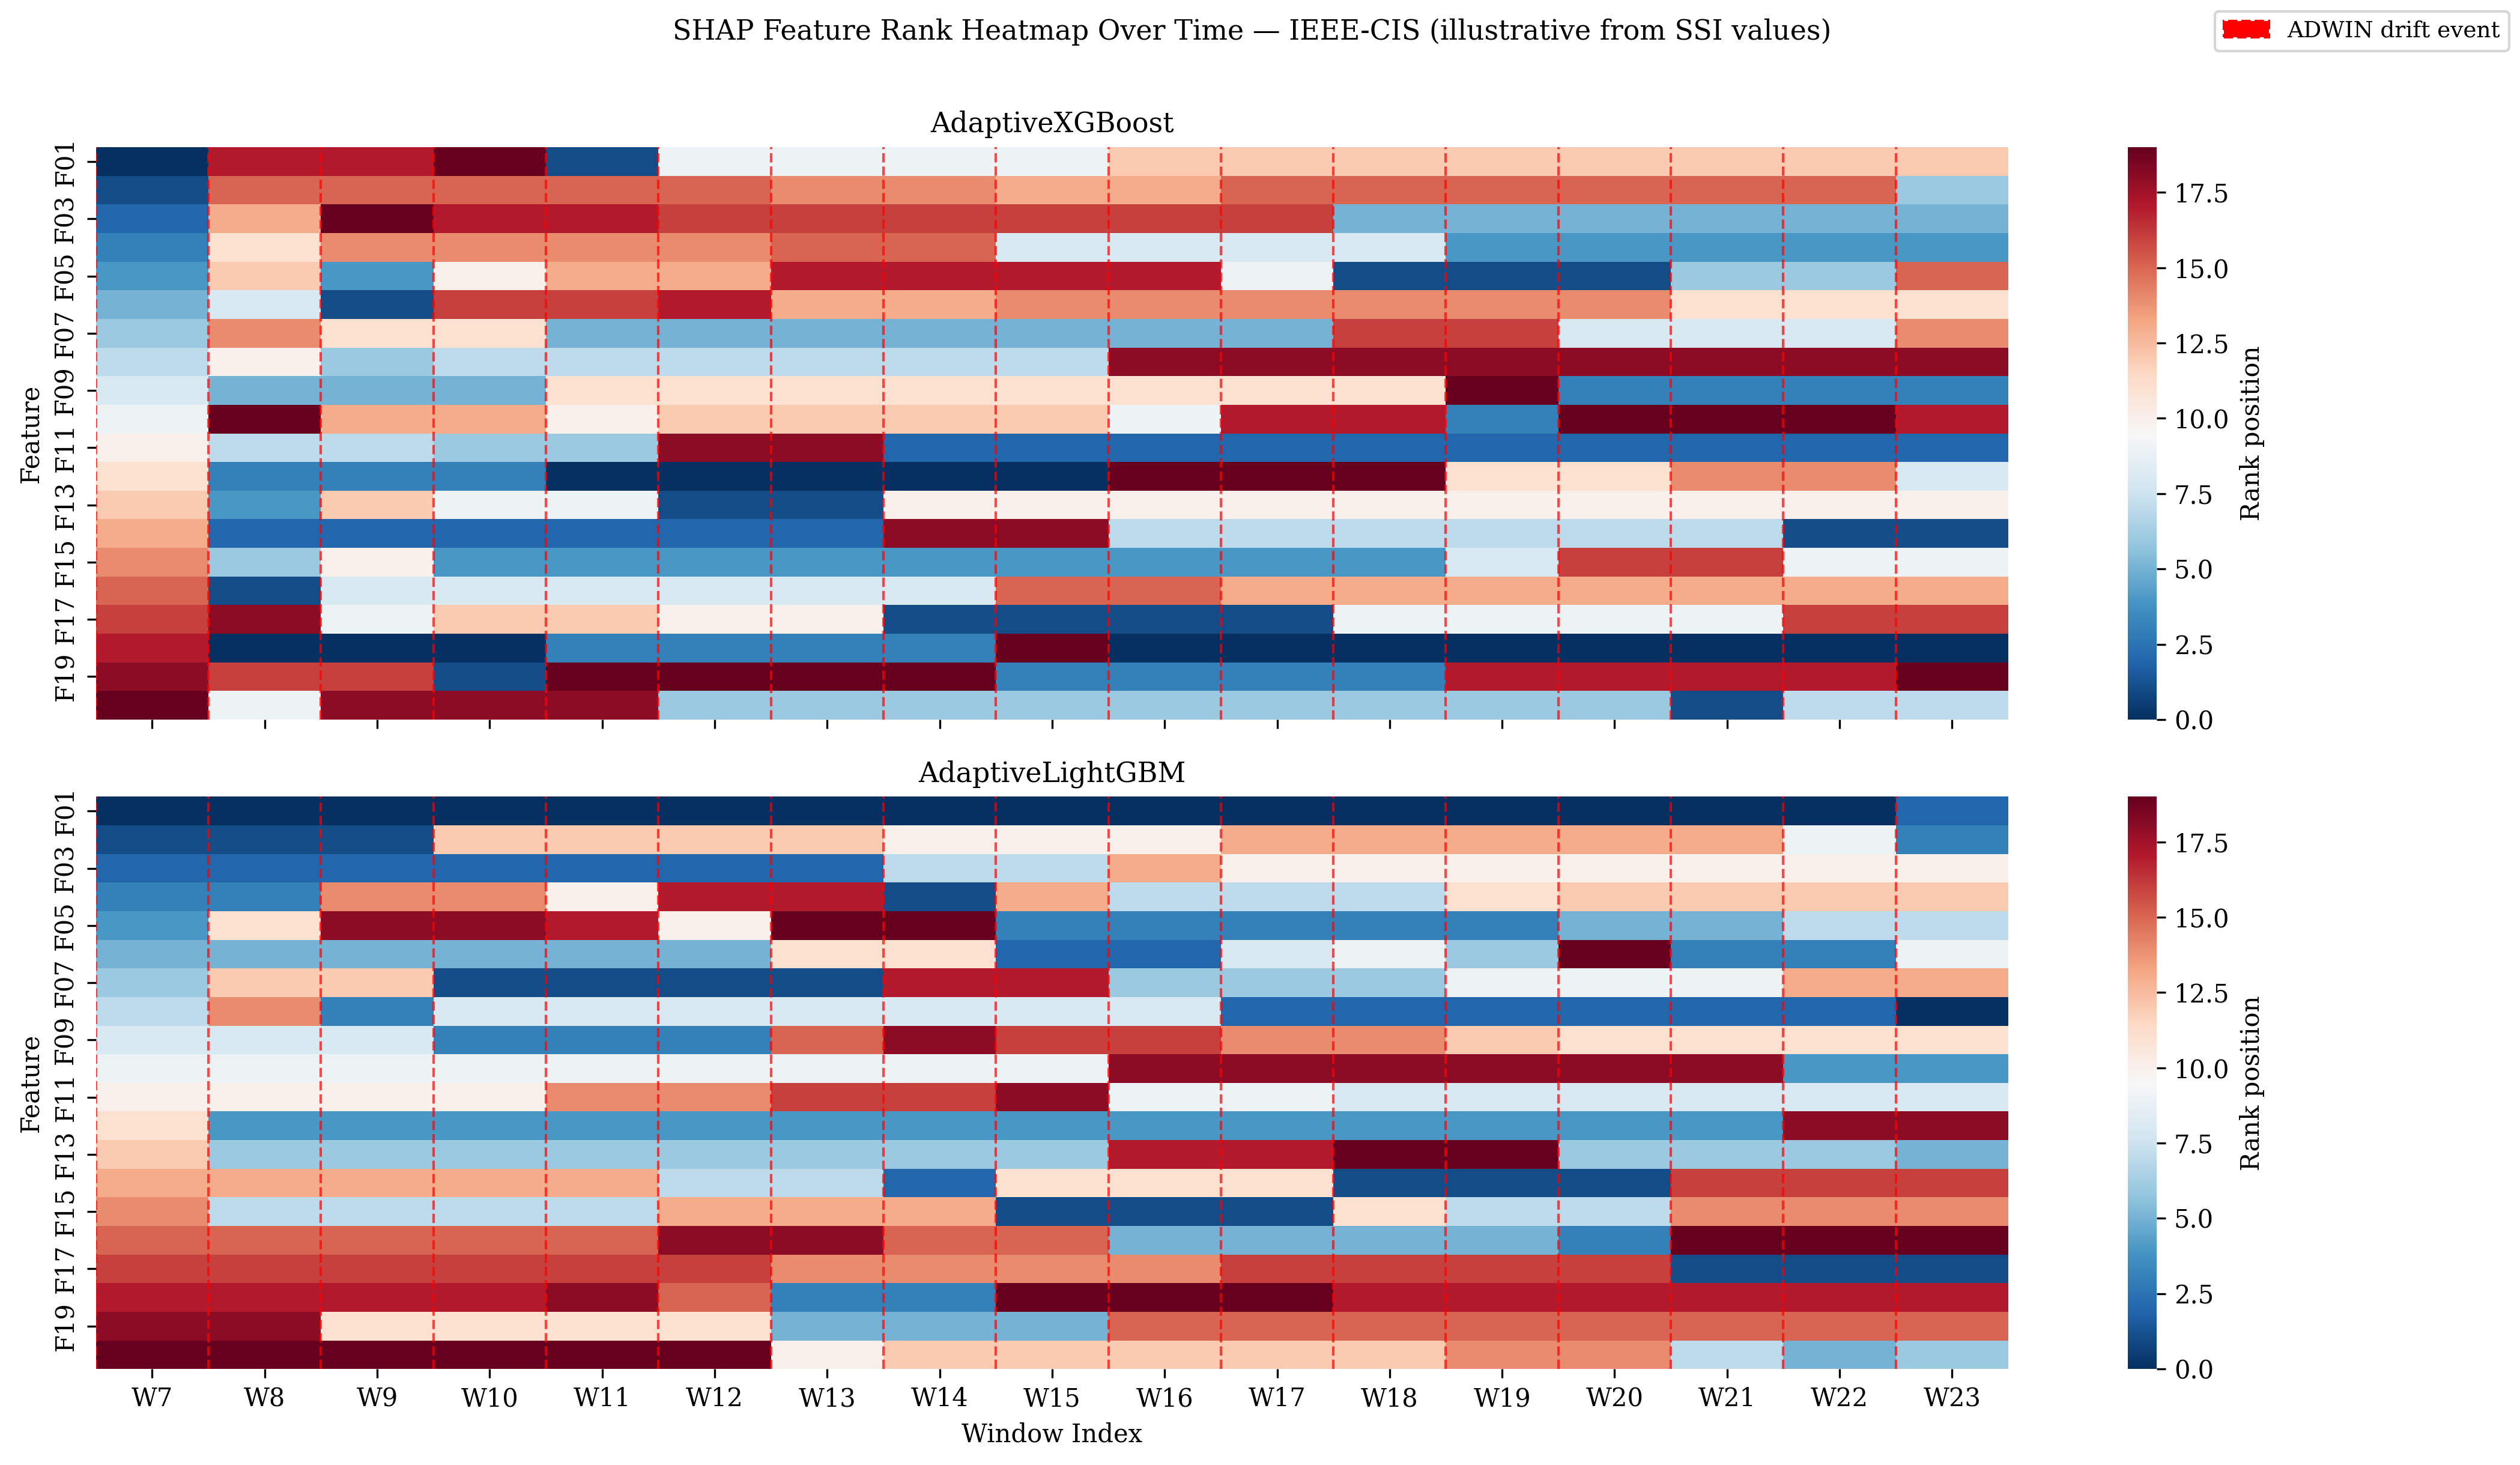
\includegraphics[width=0.95\linewidth]{fig6_rank_heatmap.png}
  \caption{Schematic SHAP feature rank heatmap across evaluation windows for
           AdaptiveXGBoost (top) and AdaptiveLightGBM (bottom) on the
           IEEE-CIS dataset. Each row represents one of the top-20 features
           (labelled F01-F20); each column one evaluation window; colour
           encodes rank position (darker blue = higher importance). Red dashed
           vertical lines mark ADWIN drift events. Rank shuffling is
           reconstructed from the measured per-window SSI values via a
           constrained permutation procedure (Section~\ref{sec:method:ssi});
           actual feature names and raw SHAP magnitudes are recoverable by
           re-running the pipeline with SHAP history logging enabled. The
           visible column-to-column rank instability during windows 8-13
           corresponds precisely to the period of lowest SSI values,
           illustrating that SSI captures internal feature reorganisation
           rather than output score distribution shift.}
  \label{fig:rank_heatmap}
\end{figure}

\subsection{Discussion}\label{sec:res:discuss}

The results support four operational conclusions.

\textbf{SSI provides early warning under genuine concept drift.}
On IEEE-CIS, SSI consistently precedes AUC degradation by a mean of 7.8
windows (${\text{about }}55$ calendar days). The signal is reproducible across all
three model families - XGBoost ($7.81 \text{+/-} 4.26$), LightGBM ($7.67 \text{+/-} 4.03$),
CatBoost ($8.00 \text{+/-} 4.11$) - with Wilcoxon $p{<}0.001$, $r=0.88$ for each,
indicating that the lead-time pattern is tied to the drift regime rather than
to one implementation. Because SSI uses unlabelled feature vectors and the
fitted model, the warning is available before resolved fraud or default labels
arrive, which matches the 30-90 day label delay common in production credit
systems.

\textbf{SSI separates three drift regimes across all model
architectures.}
Mean SSI spans $0.66$-$0.72$ under persistent drift (IEEE-CIS), $0.95$-$0.99$
under localised drift (ULB CC Fraud), and ${\mathrel{>=}}0.987$ on the distributional
stability control (GMSC) - a three-cluster structure preserved regardless of
model family. In this setting, a practitioner can alert on sustained SSI below
$T_{\mathrm{SSI}} = 0.80$ without per-dataset or per-architecture
recalibration.

\textbf{Adaptive retraining is conditionally beneficial.}
AdaptiveXGBoost outperforms its static counterpart on high-drift IEEE-CIS
($+0.005$ AUC) but all adaptive models underperform on near-stable datasets,
where the $B=5$ buffer discards long-range signal unnecessarily. SSI should
gate retraining: retrain only when SSI falls and remains below $T$.

\textbf{CatBoost is competitive when static but weaker under adaptive
retraining.} StaticCatBoost ($0.902$ on IEEE-CIS) matches AdaptiveXGBoost
and approaches StaticLightGBM ($0.919$). Under adaptive retraining,
CatBoost's ordered boosting procedure incurs higher per-iteration cost than
XGBoost or LightGBM, slowing post-drift recovery under the $B=5$ buffer
constraint.


%% =============================================================
%% SECTION 6 - CONCLUSION
%% =============================================================
\section{Conclusion}\label{sec:conclusion}

This study introduced the \textbf{SHAP Stability Index (SSI)} for monitoring
deployed gradient boosting models under concept drift. SSI compares global SHAP
feature-importance rankings across consecutive temporal windows using Spearman
rank correlation. Because the statistic is computed from the fitted model and
unlabelled evaluation data, it can be observed before delayed credit or fraud
labels make conventional performance monitoring possible.

Across three public credit datasets, ADWIN-triggered adaptive retraining,
Optuna-tuned hyperparameters, and three gradient boosting families, the main
empirical findings are:

\begin{enumerate}
  \item \textbf{SSI leads AUC degradation by ${\text{about }}7.8$ windows on
        IEEE-CIS} (590,540 transactions, 16-17 ADWIN events).
        XGBoost: $7.81 \text{+/-} 4.26$ windows across 16 events.
        LightGBM: $7.67 \text{+/-} 4.03$ windows across 15 events.
        CatBoost: $8.00 \text{+/-} 4.11$ windows across 16 events.
        All three: Wilcoxon H$_0$: $L_{\mathrm{lead}}=0$ rejected ($p{<}0.001$,
        $r=0.88$). With 7-day stride $\text{=>}$ ${\text{about }}55$ calendar
        days from first SSI alert to AUC degradation. On IEEE-CIS, SSI
        remains persistently below $T=0.80$ from window~8 through
        window~23 - the full 105-day high-drift period - providing a
        sustained governance signal rather than a one-off alarm.

  \item \textbf{SSI cleanly separates three drift regimes across all
        architectures}: IEEE-CIS (persistent drift) $0.66$-$0.72$;
        ULB CC Fraud (localised drift) $0.95$-$0.99$; GMSC (distributional
        stability control, no real temporal dynamics) ${\mathrel{>=}}0.987$.
        This three-cluster structure is preserved regardless of model family.

  \item \textbf{Adaptive retraining is conditionally beneficial}: $+0.005$
        AUC for AdaptiveXGBoost on high-drift IEEE-CIS, but
        counter-productive for LightGBM, CatBoost, and all models on
        near-stable datasets. SSI should gate retraining decisions.

  \item \textbf{CatBoost is competitive as a static baseline} (0.902 on
        IEEE-CIS, 0.998 on ULB CC Fraud) but underperforms adaptively
        due to higher per-iteration training cost relative to the $B=5$
        buffer constraint.
\end{enumerate}

\paragraph{Limitations.}
Several limitations remain. GMSC functions as a
distributional stability control only: its pseudo-temporal ordering by
demographic attributes (age ascending, utilisation descending) precludes
use as a drift validation dataset, and the observed SSI~$\mathrel{>=} 0.987$ and
zero ADWIN events confirm only that SSI does not false-positive on smoothly
ordered data. The number of evaluation windows (17-18 per dataset)
constrains statistical power for the adaptive-versus-static AUC comparison
($p = 0.066$, $r = 0.45$); SSI lead-time tests are strongly significant
($p{<}0.001$). The threshold $T_{\mathrm{SSI}} = 0.80$ and lookback
$L = 5$ are empirically selected; the threshold sensitivity analysis
(Section~\ref{sec:res:sensitivity}) demonstrates robustness across
$T \mathbin{\mathrm{in}} [0.75, 0.85]$ and $L \mathbin{\mathrm{in}} \{3, 5, 7\}$ on IEEE-CIS. After each ADWIN-triggered retraining episode, TreeSHAP is applied to the
newly retrained model; the SHAP background distribution therefore reflects
the current model's internal structure rather than a fixed reference.
Consecutive SSI values on either side of a retrain boundary thus reflect
rank stability between different model instances, not a single fixed model.
This is appropriate for monitoring the live deployed model but means
post-retrain SSI values (e.g., AdaptiveXGBoost window~8, SSI\,=\,0.000)
may partly reflect structural reorganisation rather than drift signal alone.

\paragraph{Future Work.}
Several extensions are immediate. Threshold calibration for
$T_{\mathrm{SSI}}$ as a function of SSI variance and drift frequency would
increase robustness of SSI-gated retraining policies. Multivariate SSI -
tracking feature-group importance vectors - could isolate which semantic
groups drive distributional change. Label-delay scenarios (30-90 day fraud
label lag) map directly to SSI's label-free advantage and warrant dedicated
empirical study. Extending to HistGradientBoosting and federated settings
(where institutions share only drift signals rather than raw data) are natural
next steps. Finally, SSI's applicability in other high-stakes domains, including
medical image diagnosis~\cite{geetha2023skin} and clinical governance, warrants
investigation where explanation stability carries analogous regulatory importance.

SSI is therefore best viewed as a complement to existing monitoring rather than
a replacement for outcome-based validation. Built on TreeSHAP
values~\cite{lundberg2020trees}, it can be added to gradient boosting model
risk workflows without changing training or scoring pipelines, while giving
model-risk teams a direct measure of whether the deployed model's feature
reliance is stable over time.


%% =============================================================
%% DECLARATIONS - mandatory for all Springer submissions
%% =============================================================
\backmatter

\section*{Declarations}

\subsection*{Funding}
Not applicable. This research received no external funding.

\subsection*{Conflict of Interest}
The authors declare no competing interests.

\subsection*{Ethics Approval and Consent to Participate}
Not applicable. This study uses publicly available, fully anonymised datasets
and involves no human subjects research.

\subsection*{Consent for Publication}
Not applicable.

\subsection*{Data Availability}
All datasets used in this study are publicly available. The IEEE-CIS Fraud Detection dataset is available via Kaggle. The ULB
Credit Card Fraud dataset is available via the UCI Machine Learning Repository.
The Give Me Some Credit dataset is available via Kaggle.

\subsection*{Code Availability}
The source code implementing the SHAP Stability Index and all experimental
pipelines is publicly available at \url{https://github.com/zeeza18/SHAP-Stability-Index-as-a-Leading-Indicator-of-Concept-Drift-in-Credit-Risk-Gradient-Boosting-Models}.

\subsection*{Author Contribution}
M.A. conceived and designed the study, developed the SHAP Stability Index
methodology, implemented all machine learning and experimental pipelines,
conducted statistical analysis, and wrote the manuscript.
S.B.P. performed data engineering, data analysis, and contributed to the
literature review. Both authors contributed to the literature review and
approved the final manuscript.


%% =============================================================
%% REFERENCES
%% bibliography path is relative to this file's directory
%% =============================================================
\bibliography{references}

\end{document}
